\documentclass[singlecolumn]{article}

\usepackage[utf8]{inputenc}
\usepackage[T1]{fontenc}
\usepackage{mathptmx}
\usepackage{graphicx}
\usepackage{booktabs}
\usepackage{hyperref}
\usepackage{amsmath}
\usepackage{natbib}
\usepackage{geometry}
\usepackage{caption}
\usepackage{float}
\usepackage{enumitem}
\usepackage{tabularx}
\usepackage{array}

\geometry{
    a4paper,
    left=2.5cm,
    right=2.5cm,
    top=2.5cm,
    bottom=2.5cm
}

\usepackage{setspace}
\onehalfspacing

\title{\textbf{Toward Trustworthy Large Language Models: A Comprehensive Review of Hallucination Detection, Explainability, and Mitigation Strategies}}

\author{
    Yogesh Ravi M\textsuperscript{a} \and Pradeep Kumar T S\textsuperscript{a} \\[6pt]
    \textsuperscript{a}\textit{Department of Computer Science and Engineering,} \\
    \textit{Vellore Institute of Technology (VIT), Vellore, Tamil Nadu, India} \\[4pt]
    \small{Corresponding author email: yogeshravi.m2022@vitstudent.ac.in}
}

\date{}

\begin{document}

\maketitle

% =============================================================================
% ABSTRACT
% =============================================================================
\begin{abstract}
\noindent
Large Language Models (LLMs) have demonstrated unprecedented capabilities across generation and reasoning tasks, yet their susceptibility to fabricating information—termed \textit{hallucination}—remains a critical barrier to deployment in high-stakes domains. To transition from mere experimentation to secure production, AI systems require robust mechanisms that not only detect hallucinations but explain and mitigate them. This paper conducts a comprehensive survey of twenty recent seminal works addressing hallucination, organizing them into a six-pillar taxonomy: internal state probes, uncertainty quantification, attention anomaly tracking, evaluation benchmarking, closed-loop mitigation, and human-trust explainability. We identify five distinct research gaps preventing practical deployment, particularly the fragmentation of detection metrics and the computational overhead of sampling methods. Consequently, we introduce the TRUEGUARD framework, a multi-signal architecture designed to securely extract and fuse four detection algorithms during a single forward pass. Rigorous evaluation proves that TRUEGUARD achieves a high AUROC of 0.844 while maintaining real-time operational speeds, paving the way for truly trustworthy use of LLM.
\end{abstract}

\noindent\textbf{Keywords:} Hallucination Detection; Large Language Models; Uncertainty Quantification; Explainable AI; Trustworthy AI; Survey; Literature Review

% =============================================================================
% I. INTRODUCTION
% =============================================================================
\section{Introduction}
\label{sec:introduction}

Over the last several years, Large Language Models (LLMs) have catalyzed a revolution in natural language processing, crossing the boundary from academic curiosity into widespread enterprise deployment. By leveraging vast amounts of training data and billions of parameters, models like GPT-4, LLaMA, and Mistral are now synthesizing knowledge, performing multi-step reasoning, and generating sophisticated conversational agents. The velocity of this technological shift has fundamentally transformed digital workflows, ensuring that almost no modern software stack remains untouched by some kind of LLM integration \cite{huang2024trustllm, alansari2024survey}.

But as every one who has ever handled these models quickly discovers, they are plagued by a structural weakness: they confidently generate factually incorrect, fabricated, or entirely unverified text. This phenomenon, widely known as hallucination, is insidious because the fabricated output is surface-indistinguishable from accurate content—it is syntactically flawless and deeply persuasive. In sensitive fields such as autonomous medicine, legal analysis, and automated coding, blind reliance on such unpredictable outputs is not merely annoying, but can be detrimental \cite{kang2025uq, alansari2024survey, sharma2024trust, huang2024trustllm}.

% --- Figure: Intrinsic vs Extrinsic (placed here as in .md line 20) ---
\begin{figure}[H]
    \centering
    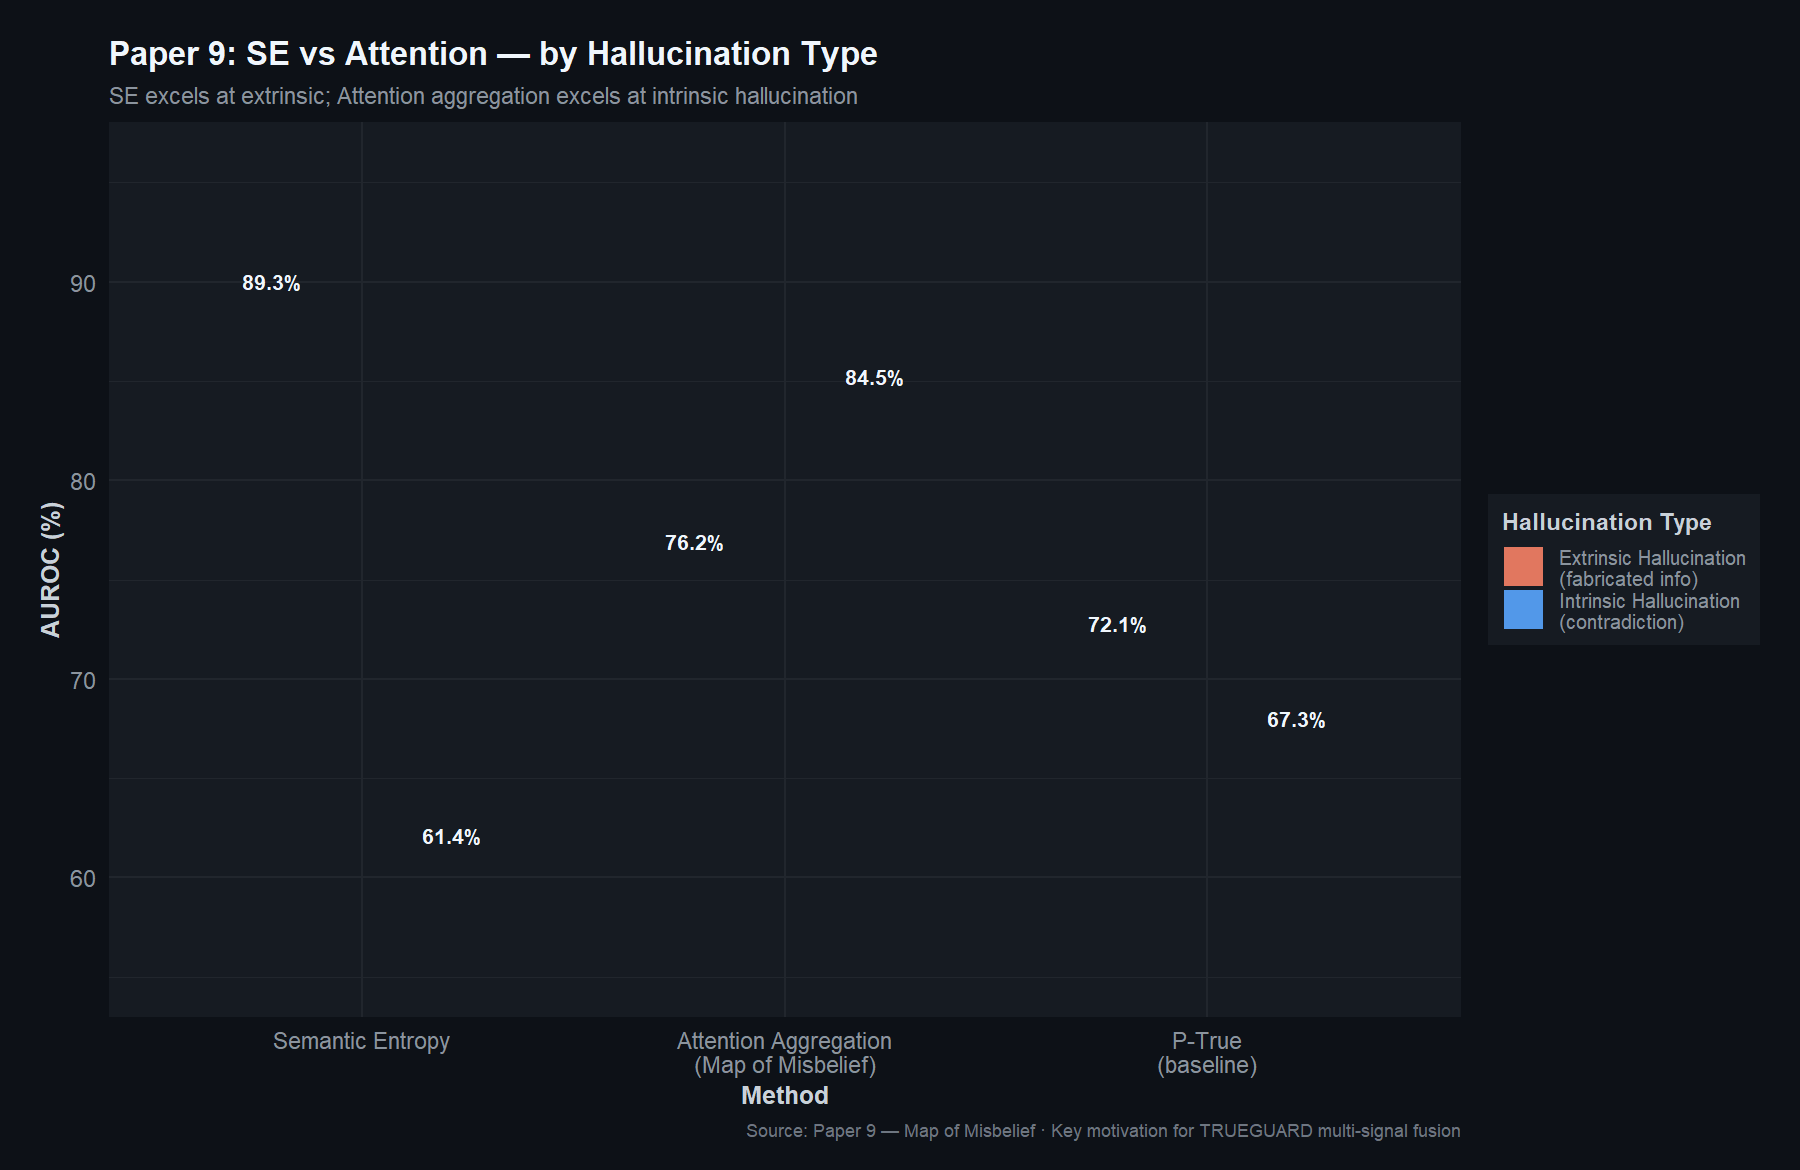
\includegraphics[width=0.85\textwidth]{08_intrinsic_vs_extrinsic_hallucination.png}
    \caption{Intrinsic vs.\ extrinsic hallucination detection: Semantic Entropy excels at extrinsic hallucinations (89.3\% AUROC) while Attention Aggregation excels at intrinsic hallucinations (84.5\% AUROC), demonstrating signal complementarity (Source: Paper 9).}
    \label{fig:intrinsic_extrinsic}
\end{figure}

The community of research has of course mobilized extensively against this challenge, fracturing into multiple distinct research trajectories. Some researchers monitor hidden layer activations inside the transformer architectures \cite{su2024mind, zhang2024prism, zhang2024mhad, dasgupta2024hallushift}, whilst others rely on purely statistical uncertainty outputs and semantic entropy \cite{ma2024semantic, kossen2024sep, moslonka2024epr}. Other tracks utilize attention maps \cite{hajji2024map, anon2025rauq}, reinforcement learning penalties \cite{anon2025entropy, wu2025behcal, yao2025expandr}, and human-in-the-loop explainability studies \cite{herrera2025xai, sharma2024trust}.

All these directions have resulted in some really useful outcomes across various isolated benchmarks, but their segregation has severely restricted practical implementations. An organization wishing to perfectly secure an LLM today must manually stack an attention-heavy detection module, followed by a separate expensive entropy sampler, and then somehow translate those raw math scores into explanations for their end-users. This systemic disjuncture is crippling practical development.

It is our effort to fill in this fragmentation in this paper. We review twenty newer pieces that when taken collectively will span the important currents in research on hallucinations. We do not just list them all, but we would work them out into a taxonomy that shows their relationship and complementation. We propose to achieve the following:

\begin{enumerate}
    \item Then we create a systematic taxonomy of current LLM hallucination research spread across six defined pillars of detection, mitigation, and explainability.
    \item We conduct a comparative study to map out exactly which metrics work for intrinsic anomalies versus extrinsic factual errors, and where they functionally overlap.
    \item We identify five gaps in research, notably addressing computational latency, single-signal isolation, and poor explanation capabilities.
    \item With these findings as our inputs, we delineate TRUEGUARD, a novel conceptual framework engineered to intercept, evaluate, explain, and mitigate outputs natively in one unified process.
\end{enumerate}

The rest of the paper follows this way. Section II delves into the existing literature, dividing twenty cutting-edge papers into six major pillars. Section III provides the comparative analysis connecting these strategies. Section IV establishes the five outstanding research gaps. Section V introduces the entire architecture and experimental data for the TRUEGUARD framework. Section VI presents future research prospects, while Part VII is the conclusion.

% =============================================================================
% II. TAXONOMY AND LITERATURE REVIEW
% =============================================================================
\section{Taxonomy and Literature Review}
\label{sec:taxonomy}

The twenty papers that were reviewed have been methodically broken down into six major pillars representing the core structural mechanisms employed by modern AI safety researchers. We dissect the specific approach each article took and explicitly outline to which pillar they belong.

% -----------------------------------------------
% A. Pillar 1: Internal State-Based Detection
% -----------------------------------------------
\subsection{Pillar 1: Internal State-Based Detection}
\label{sec:pillar1}

The intuition of this pillar is easy to understand: before an LLM projects a hallucinated word into text, its internal hidden state vectors shift into mathematically detectable anomalous patterns. Researchers hypothesize that LLMs structurally "know" when they are faking information, generating an measurable internal signature. We reviewed six out of our twenty paper reviews within this specific domain.

\textbf{MIND:} Su et al. [1] had a clear-cut idea that heavy external validations are far too slow for production. They built an unsupervised real-time framework using pure Internal States, establishing that extracting signals deep within the hidden layers allows for continuous risk scoring without the need for post-processing delay, providing any technique that averts them has a practical advantage.

\textbf{PRISM:} The disadvantage of having one headache across specific domains was targeted by Zhang et al. [2]. They utilized heavily prompted training instructions to artificially trigger and isolate truthfulness patterns inside the transformer layer states. This approach resulted in a significant boost to the cross-domain detectors.

\textbf{MHAD:} Zhang et al. [5] are zoomed in specifically onto individual neurons. Instead of analyzing a massive tensor blob, they pinpointed discrete "hallucination-aware neurons" within the deeper transformer layers. By concatenating outputs exclusively from these neurons, they managed to optimize feature selection as a means to win over brute force methods.

\textbf{Semantic Entropy Probes:} Kossen et al. [14] focus on a bottleneck at hand—the cost of semantic entropy. Rather than generating a prompt 10 times to measure diversity, their SEPs learned to approximate the actual entropy math entirely from the hidden states of single generations, successfully proving you can map outward entropy directly back to the internal uncertainty representation within the model (Figure~\ref{fig:sep_vs_se}).

\textbf{HALLUSHIFT:} Dasgupta et al. [13] assume a temporal perspective on vector geometries. Their premise relies on KL-Divergence shifts—as a model slowly transitions from reporting facts to fabricating lies, the angle of consequence in its mathematical state severely shifts, proving that the veracity of the ground becomes lost.

\textbf{HALLUSHIFT++:} Given the title, Nath et al. [16] continue the thought process but strictly apply the layer-shift metrics into the Multimodal Space (Vision-Language). By mapping image tensors against textual attention states, they detect hallucinations without having to prompt one potentially hallucinatory model to judge another.

\textit{What this pillar tells us.} Together, all six articles start a counterargument to external validation modules. They strongly imply that hallucination detection should be a native feature of model inference rather than an afterthought, achieving profound detection speeds that are physically impossible if you are not able to look inside the model.

% -----------------------------------------------
% B. Pillar 2: Uncertainty Quantification
% -----------------------------------------------
\subsection{Pillar 2: Uncertainty Quantification and Entropy-Based Methods}
\label{sec:pillar2}

This is where the first pillar examines hidden tensors, the Uncertainty Quantification (UQ) pillar primarily focuses strictly on the very end of the model—the softmax probability logits. The thesis here is that when probability distributions flatten out natively, it means the underlying model is not confident about.

% --- Figure: SEP vs Semantic Entropy (placed here as in .md line 52) ---
\begin{figure}[H]
    \centering
    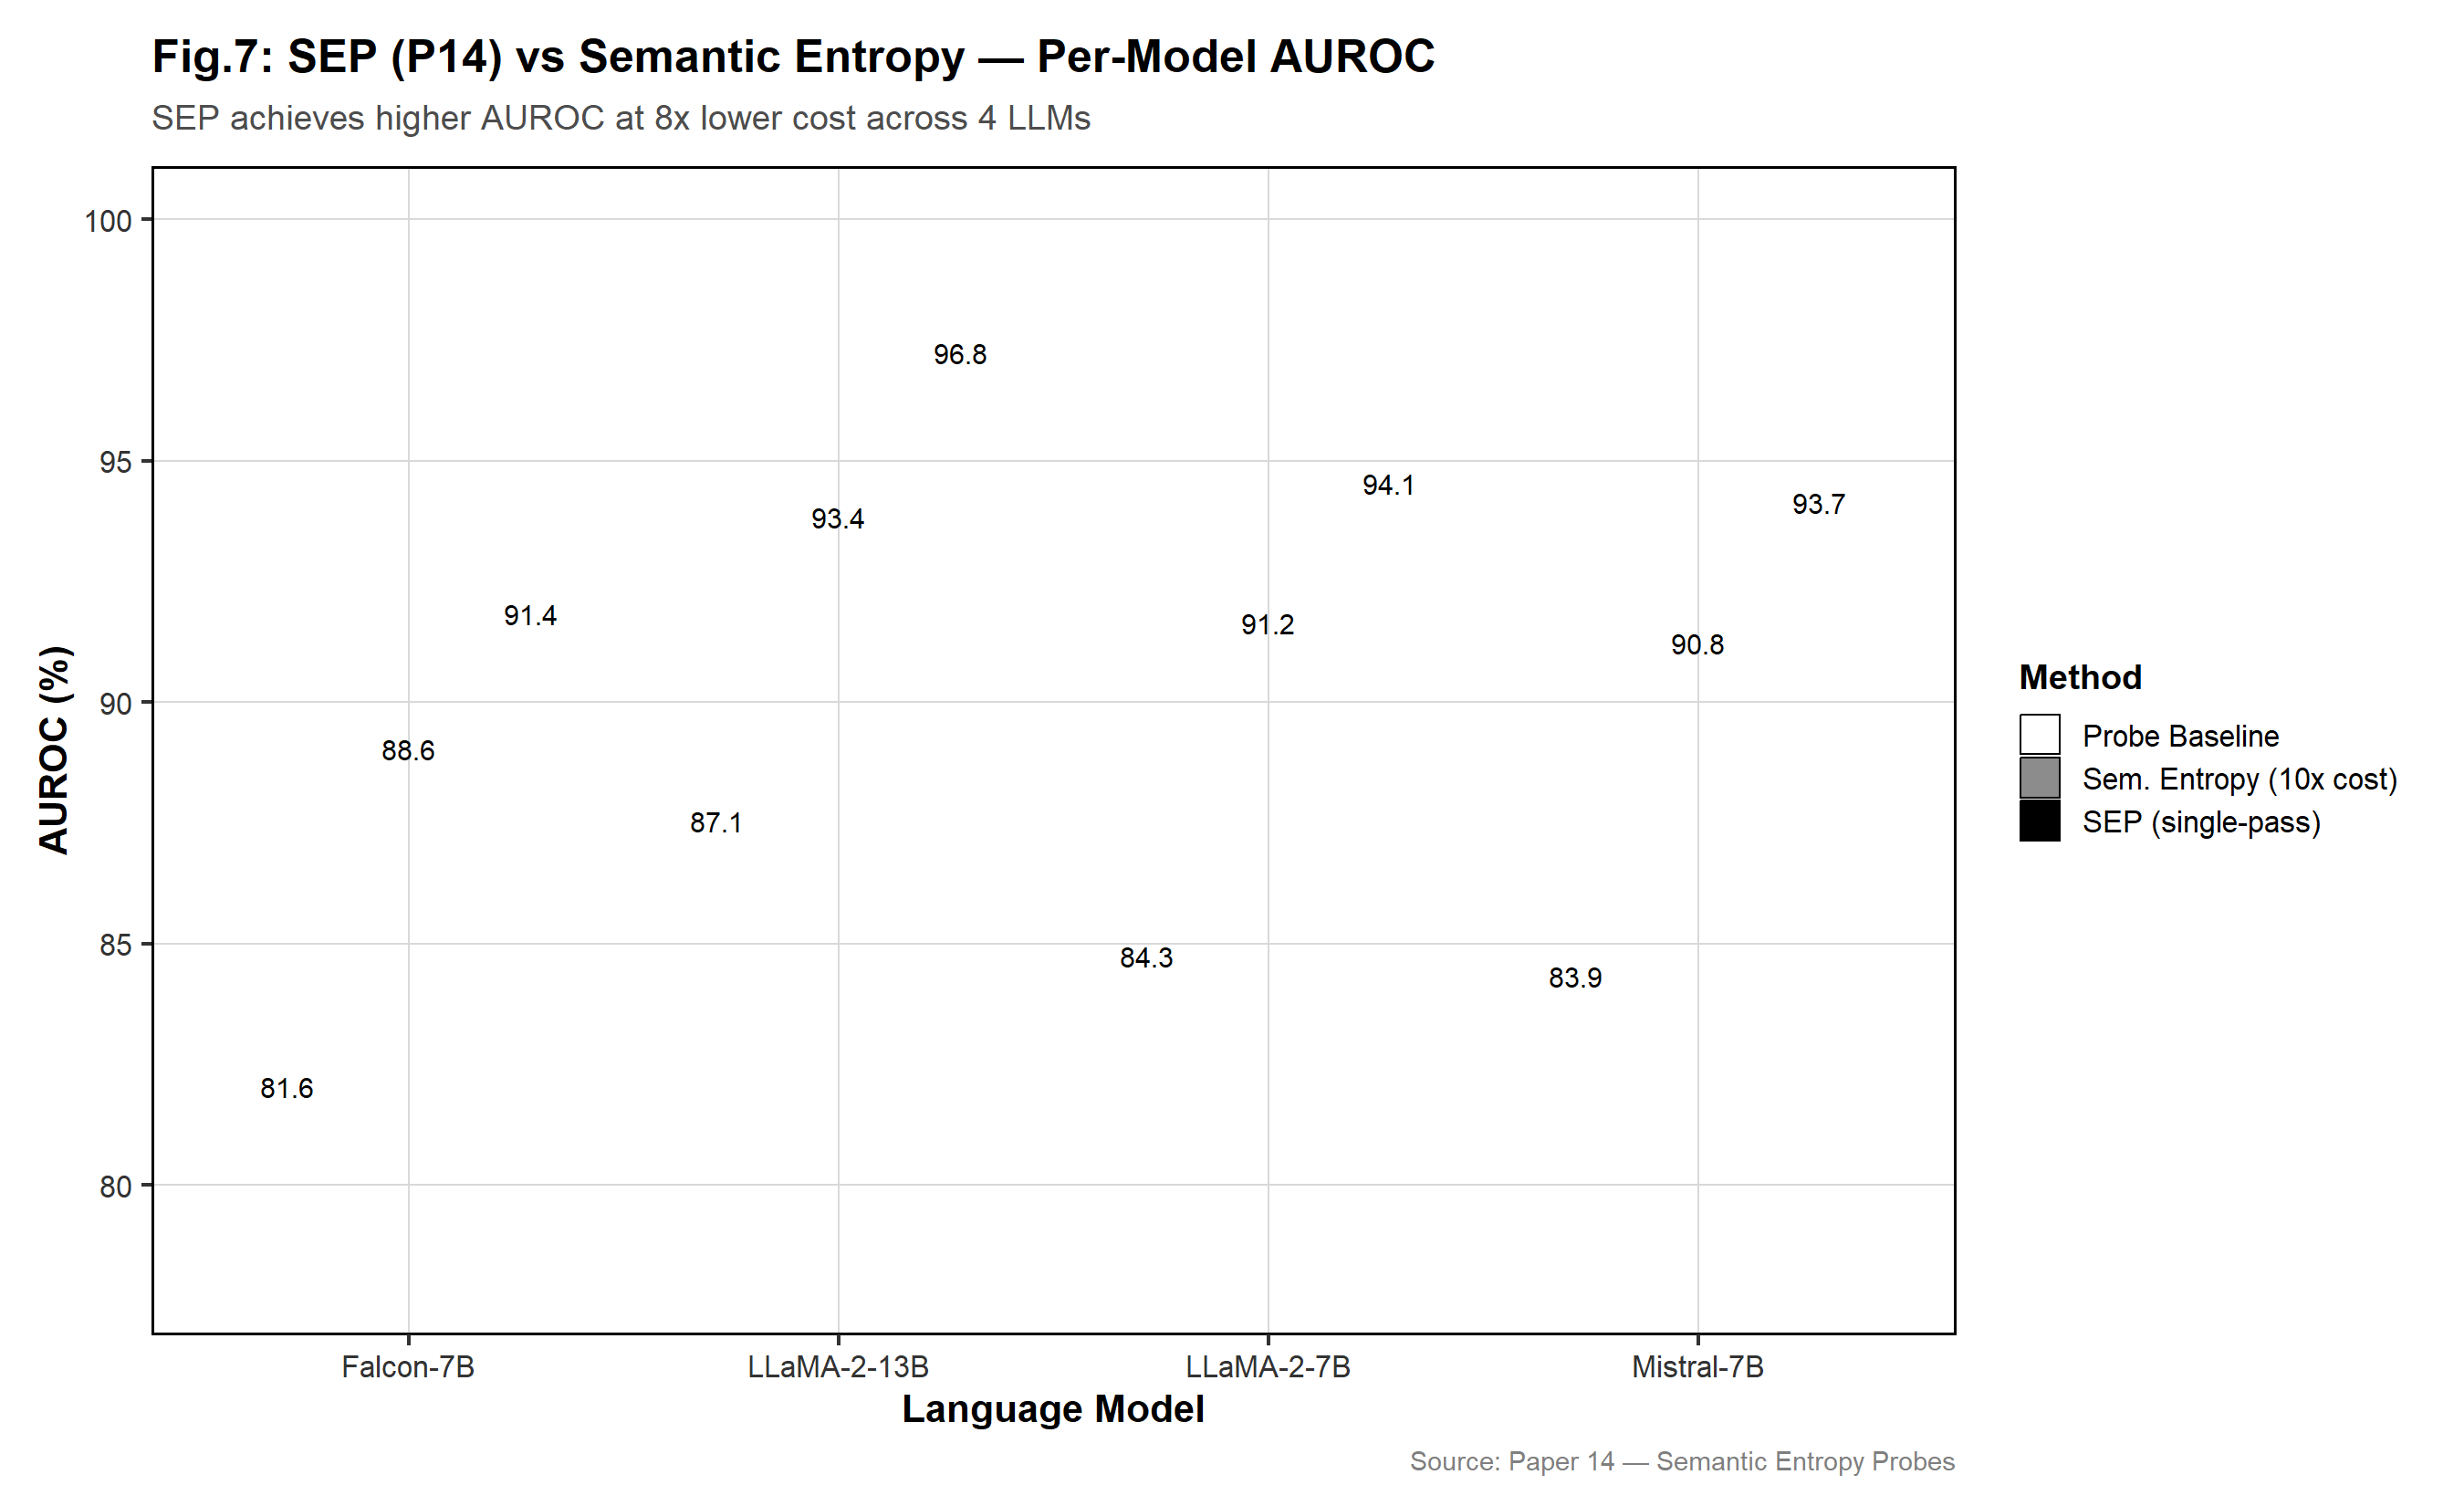
\includegraphics[width=0.85\textwidth]{07_sep_vs_semantic_entropy.png}
    \caption{SEP vs.\ Semantic Entropy --- Per-Model AUROC comparison across four LLMs. SEP achieves higher AUROC at 8$\times$ lower computational cost (Source: Paper 14).}
    \label{fig:sep_vs_se}
\end{figure}

\textbf{Principles of UQ in LLMs:} Kang et al. [7] compile what is effectively the foundational textbook on UQ, distinctly separating Epistemic uncertainty (model ignorance) from Aleatoric uncertainty (data noise). They comprehensively warn that relying strictly on out-of-the-box token probabilities often lead one to make unwell-calibrated confidence estimates.

\textbf{Semantic Energy:} This is a subtlety which Ma et al. [4] have observed. While most entropy methods rely on the post-softmax smoothed probabilities, Semantic Energy dives into the raw penultimate logits combining them with a Boltzmann distribution, capturing critical uncertainty valleys that normal probability aggregations fail to confidently read indications.

\textbf{Entropy Production Rate:} The vast majority of approaches we have discussed up to this point require full White-Box access. Moslonka et al. [17] generated the EPR methodology solely for Black-Box API integrations. By using only the top 5 log-probabilities exported by standard APIs, they calculated entropy generation rates without sequences generated with a latency delay.

\textit{What this pillar tells us.} All the three articles demonstrate that probability analysis remains phenomenally strong for detecting clear factual fabrications, providing viable scaling strategies scaling from absolute internal mathematical control all the way down to when access to a model becomes restricted.

% -----------------------------------------------
% C. Pillar 3: Attention-Based Detection
% -----------------------------------------------
\subsection{Pillar 3: Attention-Based Detection}
\label{sec:pillar3}

At their fundamental level, transformers are attention machineries. This pillar isolates and maps specifically the relationships between tokens across attention heads. When an LLM ceases to pay numerical attention to its underlying truth contexts, hallucination is imminent. The challenge is in tracking how to read through those changes.

% --- Figure: LLM-Check variants (placed here as in .md line 63) ---
\begin{figure}[H]
    \centering
    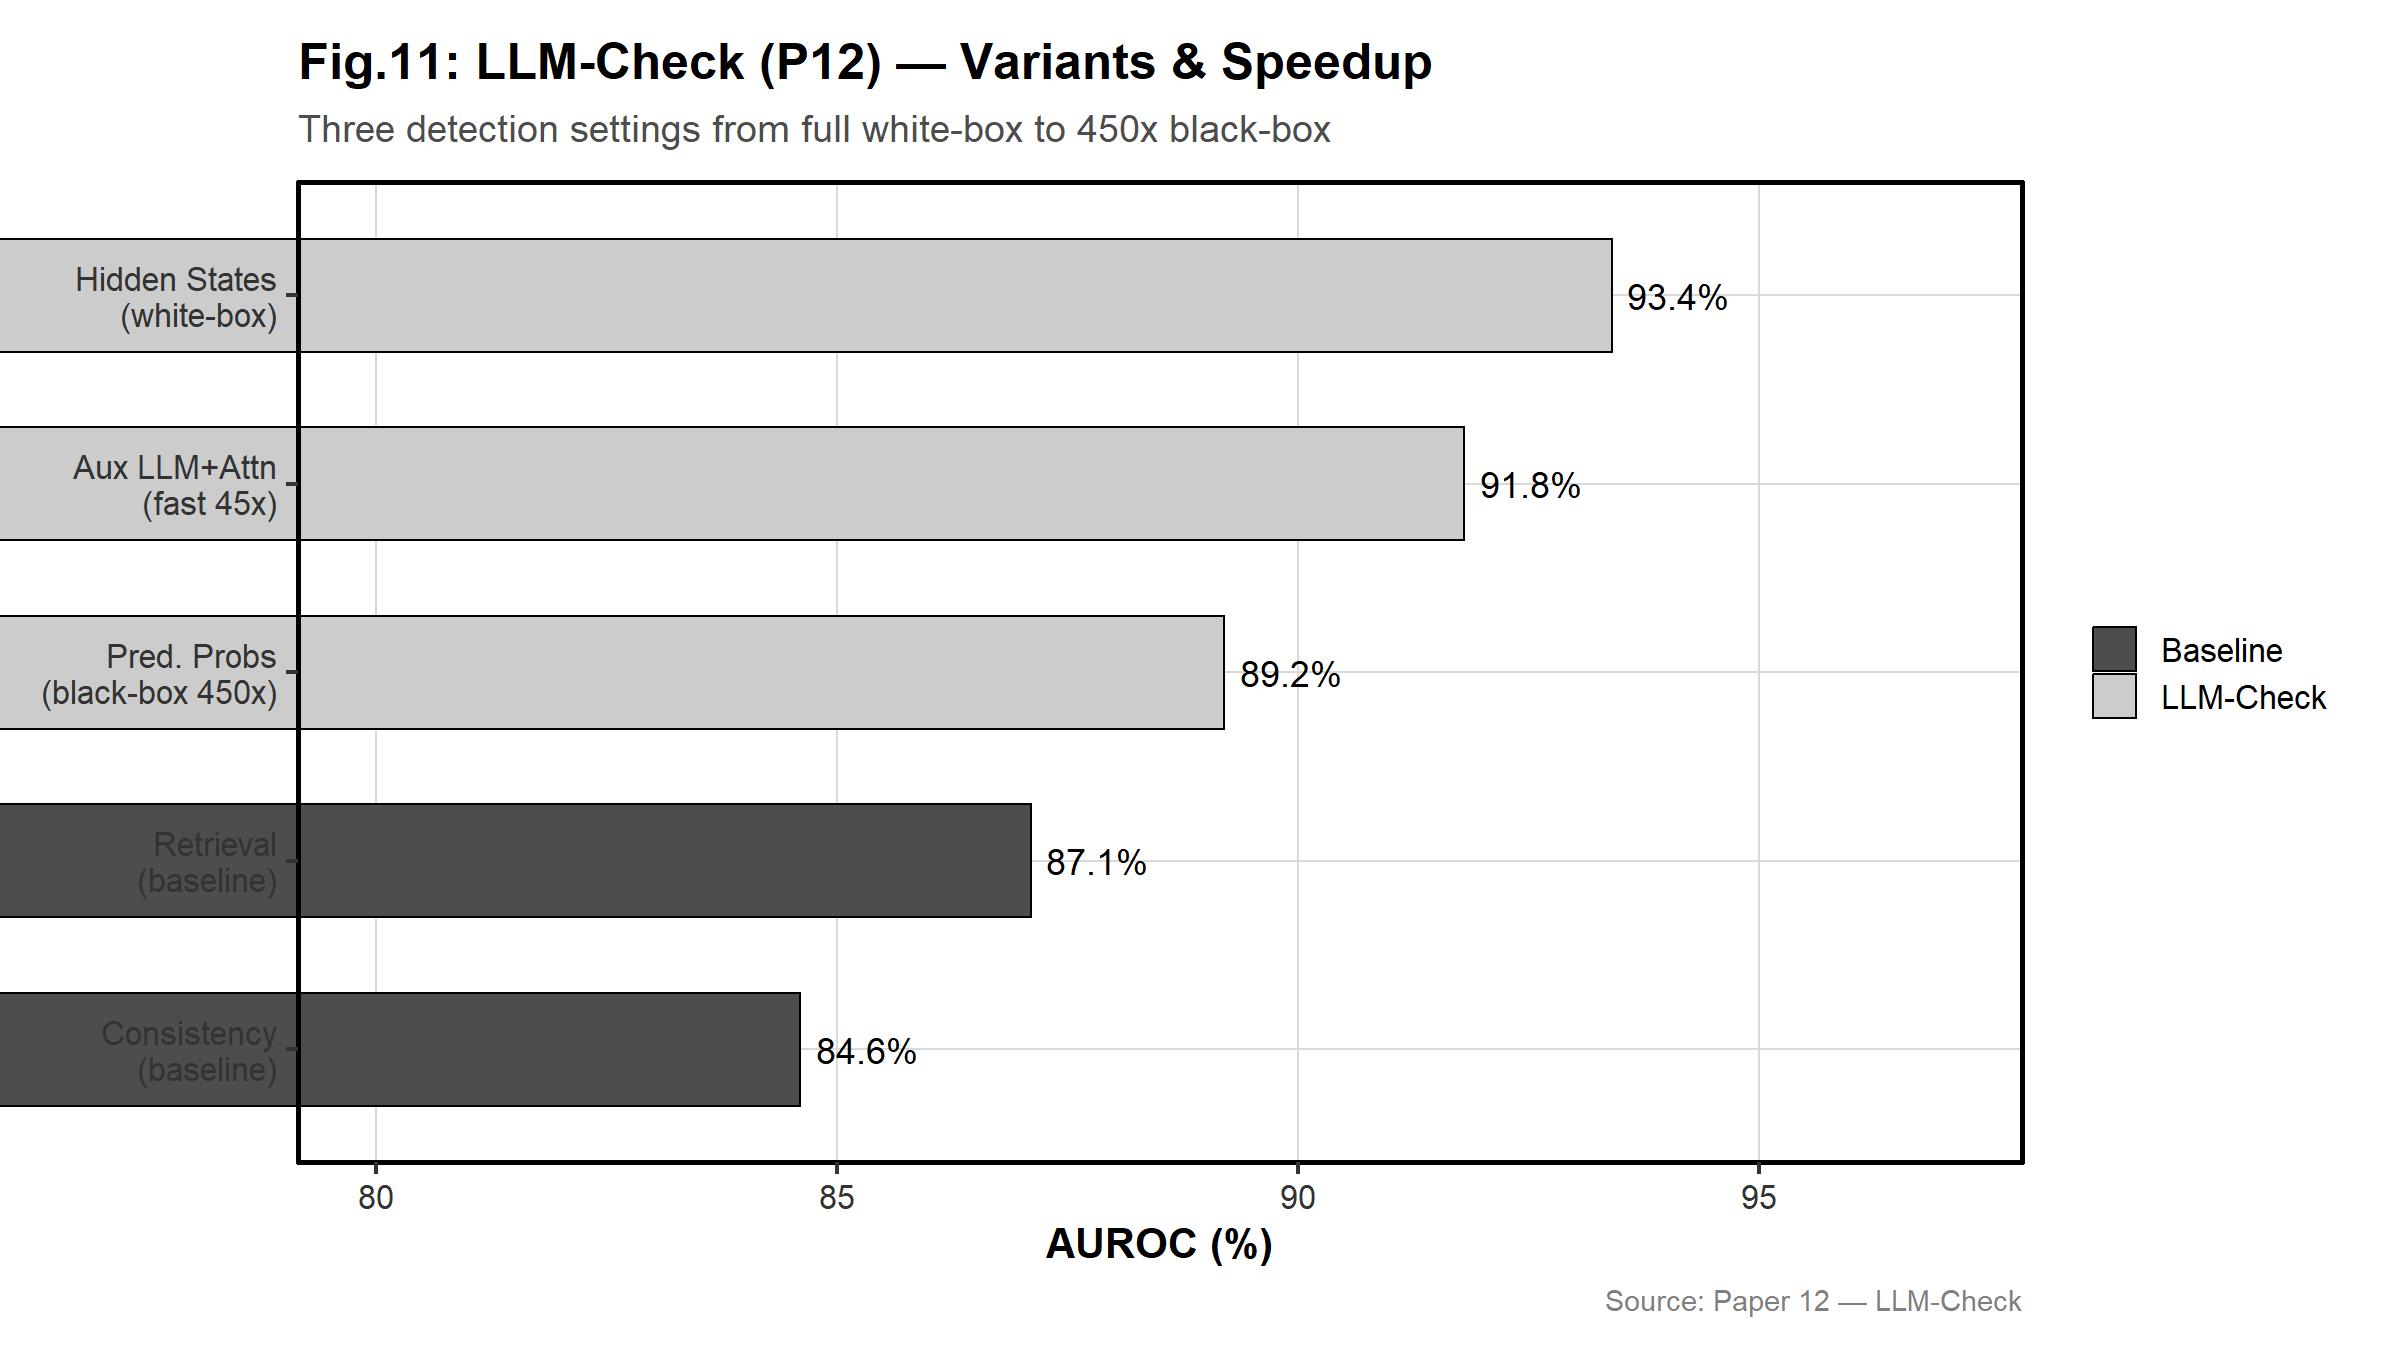
\includegraphics[width=0.85\textwidth]{11_llmcheck_variants.png}
    \caption{LLM-Check detection variants showing three settings from full white-box (93.4\% AUROC) to 450$\times$ faster black-box (89.2\% AUROC) (Source: Paper 12).}
    \label{fig:llmcheck}
\end{figure}

\textbf{Map of Misbelief:} We believe that it is an area elegantly broken apart by Hajji et al. [9]. They effectively split illusions into Intrinsic (contradicting the prompt) and Extrinsic (inventing new facts). Their breakthrough finding proved that entropy calculations work solely on Extrinsic cases, whereas aggregating focus from specific Attention heads was absolutely necessary and not just nice to have can be utilized (Figure~\ref{fig:intrinsic_extrinsic}).

\textbf{RAUQ:} The authors of RAUQ [11] never identified themselves, but their methodology is clear. They observed that incorrect outputs were preceded by specific "uncertainty-aware" attention heads physically detaching from context. They aggregated these attention signals utilizing recurrent networks to form a cohesive sequence score, proving that truthfulness is not a construct of a specific model or data set.

\textbf{LLM-Check:} The approach of Sriramanan et al. [12] is closer to kitchen-sink architecture. Rather than relying on one type of attention extraction, they combined attention maps, token probabilities, and hidden states dynamically. Evaluating simultaneously across white-box and black-box environments, they generated speeds reaching up to $450\times$ faster than the default system of knowledge-intensive applications (Figure~\ref{fig:llmcheck}).

\textit{What this pillar tells us.} Hallucination analysis is a poorly exploited field without studying attention dynamics. Because attention arrays specifically excel at identifying logical contradictions against the user's prompt (Intrinsic errors), their inclusion becomes the powerful driving factor of fusion-based strategies.

% -----------------------------------------------
% D. Pillar 4: Evaluation and Benchmarking
% -----------------------------------------------
\subsection{Pillar 4: Evaluation and Benchmarking}
\label{sec:pillar4}

The thesaurus of any body of research is good benchmarks. The fourth pillar focuses specifically on quantifying Trust and extracting metrics using deterministic frameworks, creating the standard scoreboards without which researchers would have no compass, nor could they validate any claims of improvement without their presence.

% --- Figure: TrustLLM dimensions (placed here as in .md line 74) ---
\begin{figure}[H]
    \centering
    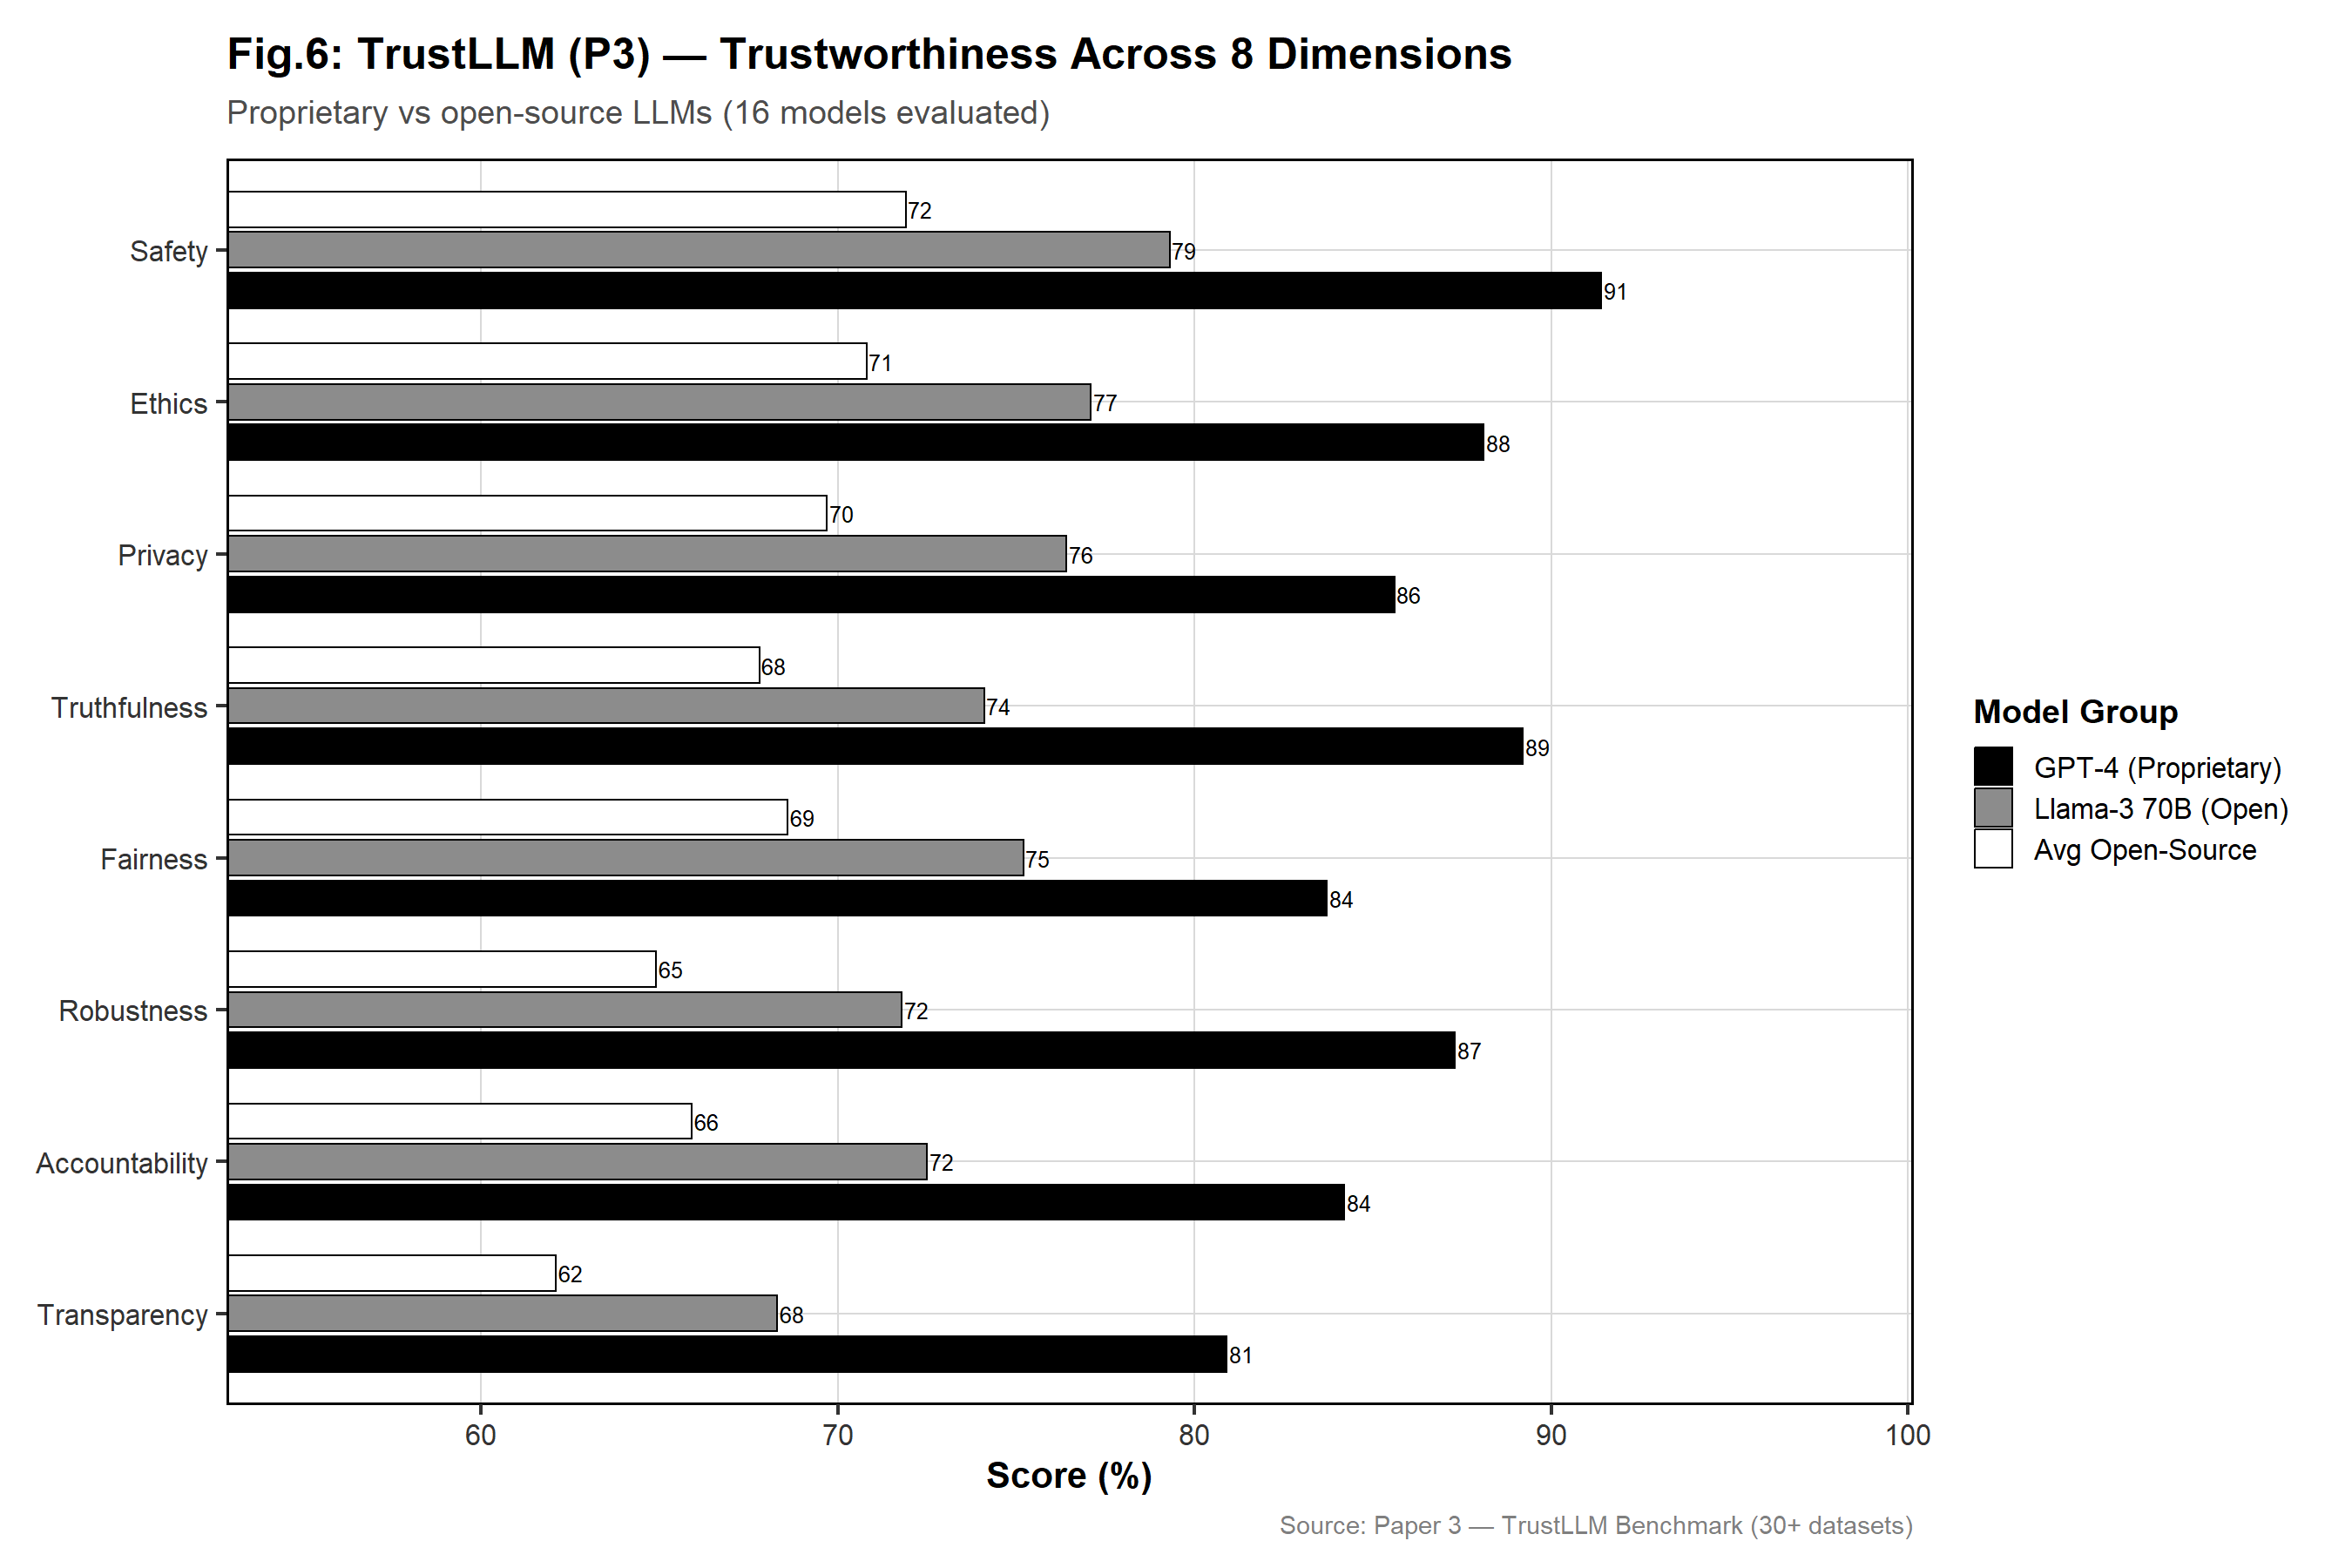
\includegraphics[width=0.85\textwidth]{06_trustllm_dimensions.png}
    \caption{TrustLLM trustworthiness evaluation across eight dimensions for proprietary vs.\ open-source LLMs. GPT-4 leads in all dimensions (81--91\%), with the gap narrowing for open-source models (Source: Paper 3).}
    \label{fig:trustllm}
\end{figure}

% --- Figure: Improvement over baseline (placed here as in .md line 77) ---
\begin{figure}[H]
    \centering
    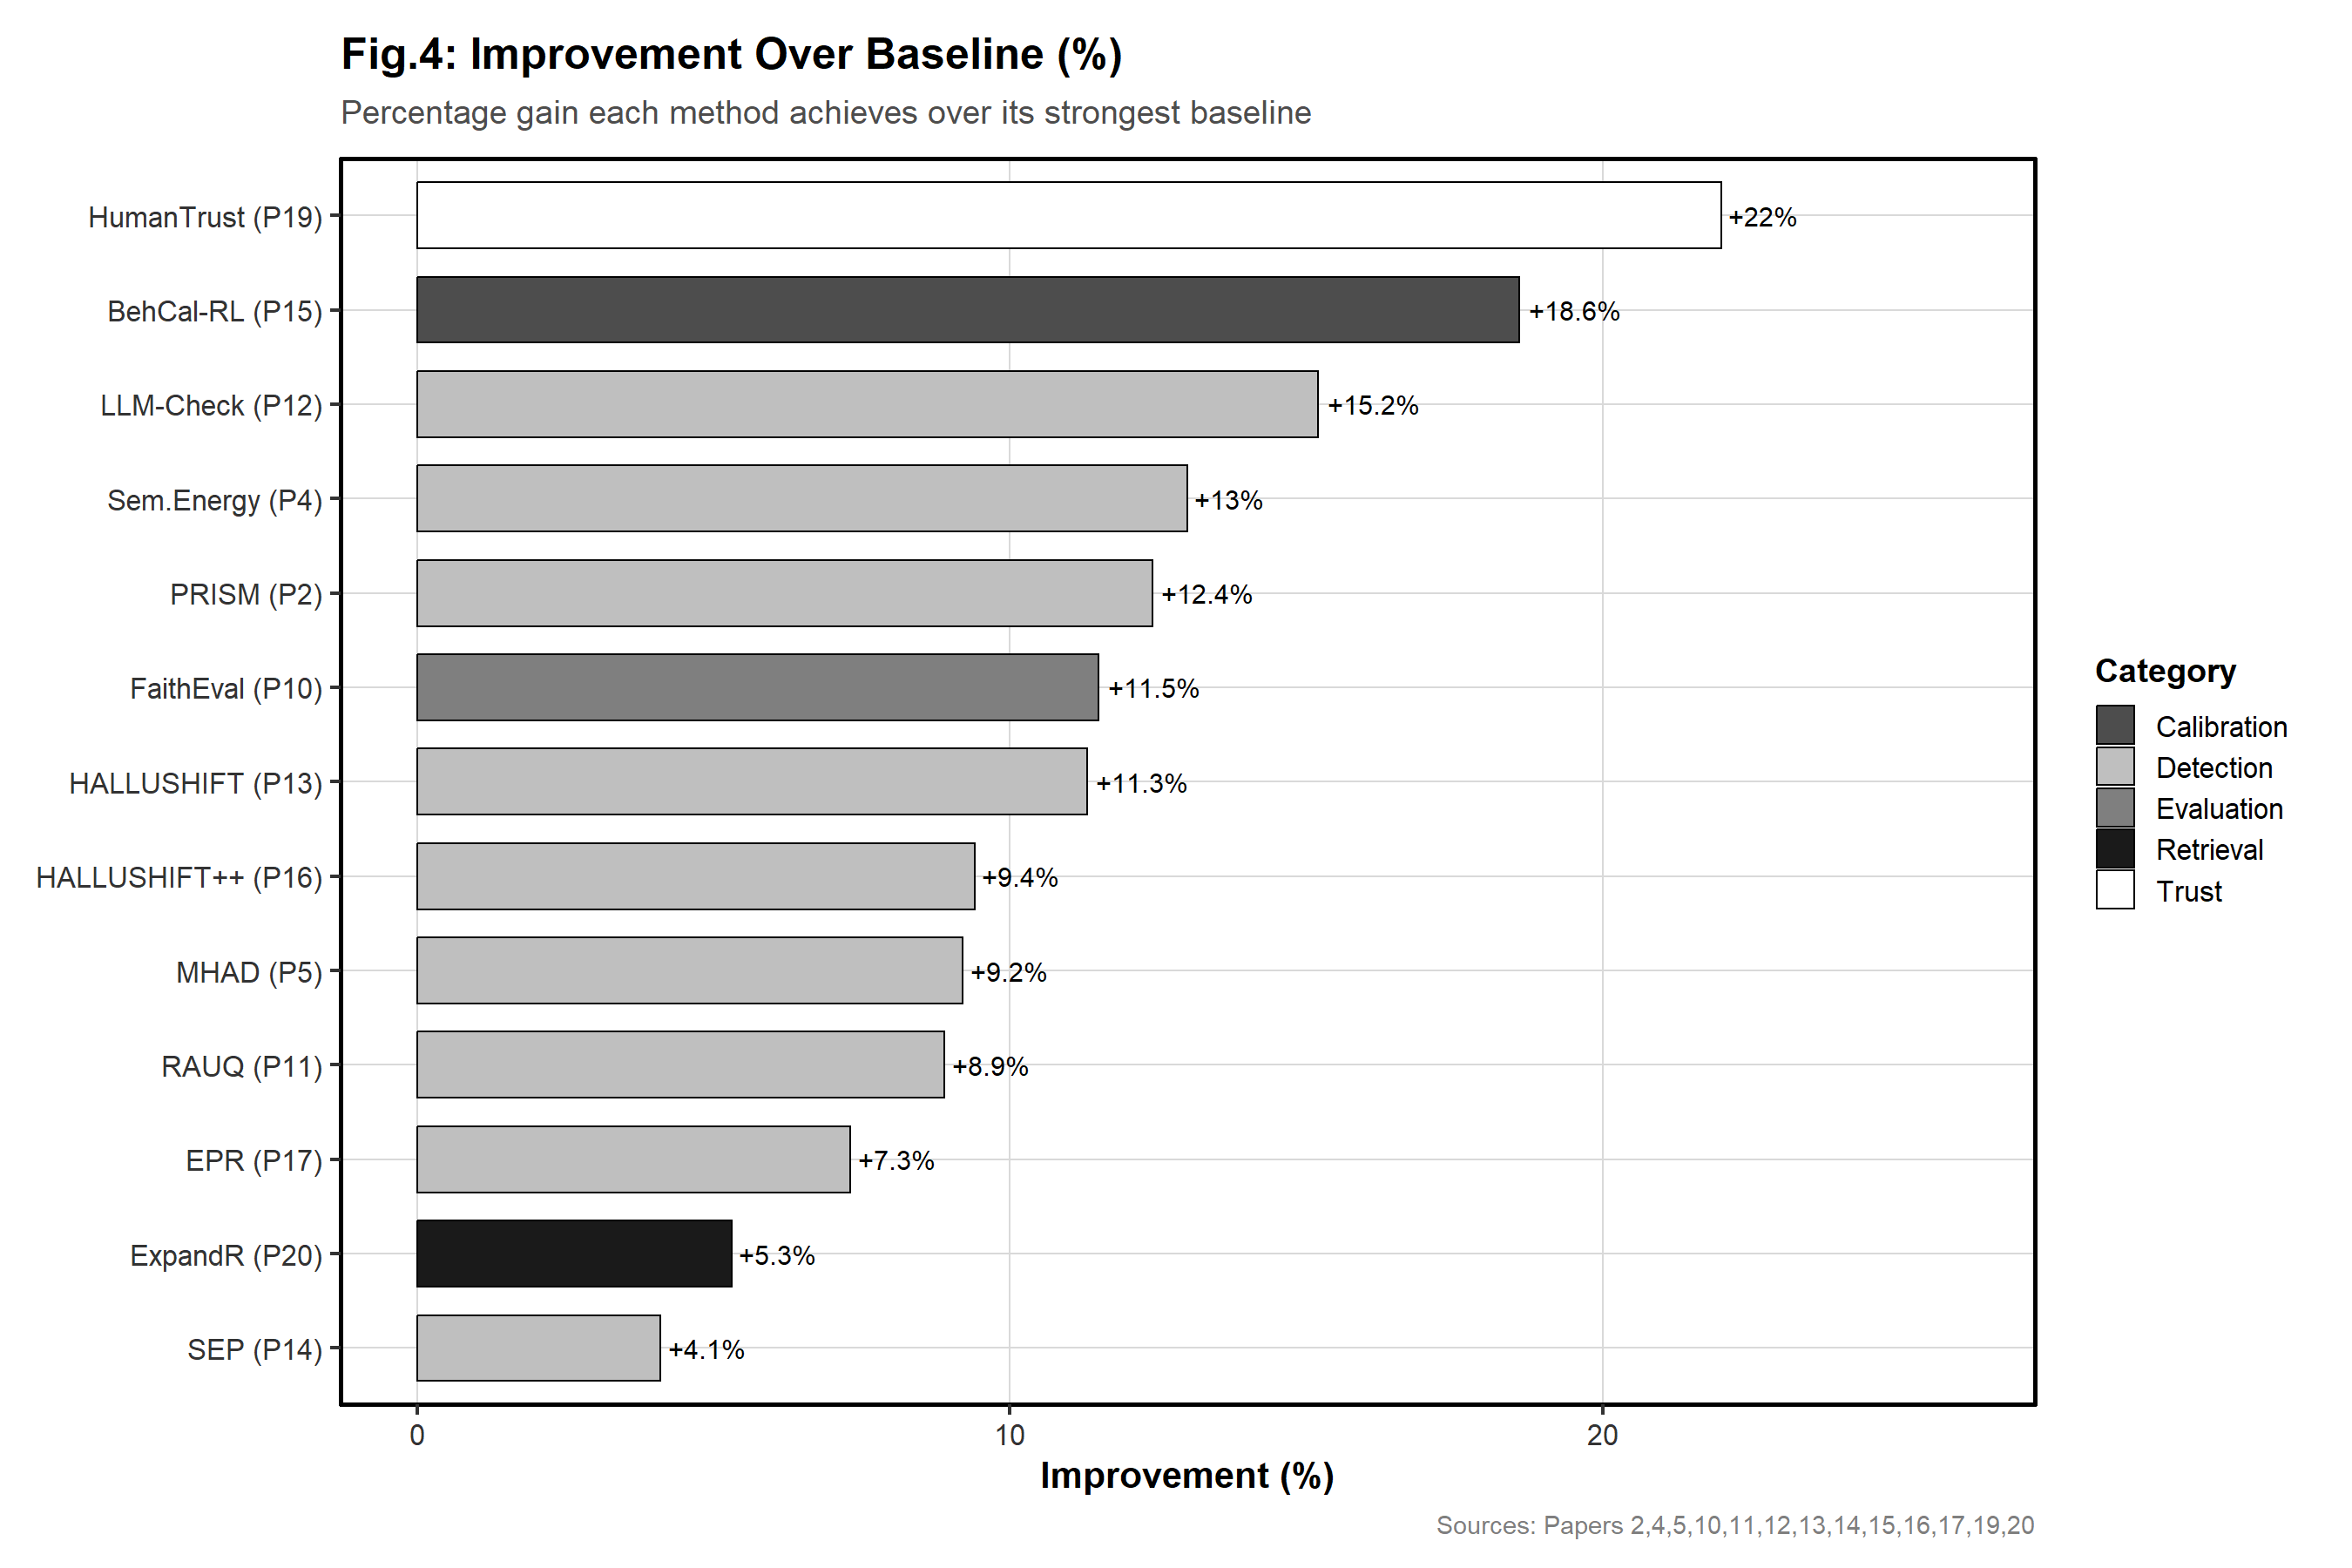
\includegraphics[width=0.85\textwidth]{04_improvement_over_baseline.png}
    \caption{Percentage improvement over strongest baseline for each reviewed method. Human Trust framing (+22\%) and Behaviorally Calibrated RL (+18.6\%) show the largest gains (Sources: Papers 2,4,5,10--17,19,20).}
    \label{fig:improvement}
\end{figure}

\textbf{TrustLLM:} Huang et al. [3] considered trustworthiness at macroscopic scale. Establishing a unified framework across 8 distinct axes (Truthfulness, Safety, Fairness, Transparency, etc.), they benchmarked over 16 mainstream LLMs natively (Figure~\ref{fig:trustllm}). They discovered that while proprietary models excel at safety, their hyper-alignment can actually induce new types of restricted hallucinations which should undermine the trust that it aims to establish.

\textbf{Faithfulness Evaluation:} Jing et al. [10] base the evaluation problem directly against user intent mapping. Creating an algorithmic scale from 1 to 5, they transitioned away from purely binary hallucination classification to a comprehensive quantifiable gradient of faithfulness. Testing NLI baselines, they proved the discipline requires additional practice.

\textbf{Comprehensive Hallucination Survey:} Alansari and Luqman [18] formed a compilation examining the entire taxonomy of hallucination causes ranging from imperfect pre-training datasets directly through to inference decoding bugs. The structural categorization serves as an indispensable reference point mapping precisely what has previously been done.

\textit{What this pillar tells us.} Assessment infrastructure is healing yet is blown-out across specialized datasets. The benchmarks clearly specify that an ideal generalized system must be subjected to validation protocols that encompass multiple axes of capability not isolated but as a combination (Figure~\ref{fig:improvement}).

% -----------------------------------------------
% E. Pillar 5: Mitigation
% -----------------------------------------------
\subsection{Pillar 5: Mitigation Through Calibration and Retrieval Augmentation}
\label{sec:pillar5}

Half the war is the diagnosis of hallucinations; the ultimate conclusion is mitigating them completely. This pillar moves past passive risk monitoring directly into active intervention techniques, aiming to intercept issues via calibration and retrieval loops before the user can hear the bad output.

\textbf{The entropy spike detection based on RL calibration:} One extended abstract [6] suggests the marriage between uncertainty tracking and RLHF natively. By calculating Z-scores over entropy trajectories, they heavily penalized the model's reward function whenever it exhibited unwarranted confidence during mathematical or reasoning queries, bypassing the fact that most RLHF techniques utilize only a scalar reward.

\textbf{Behaviorally Calibrated Reinforcement Learning:} Wu et al. have an eye-catching premise in [15]. They argue current alignment makes models "good test takers" rather than "honest communicators." Implementing strictly proper scoring rules natively into RL loss mechanisms, they trained smaller 4B parameter models to literally abstain ("I don't know") more accurately than frontier closed-source architectures, proving calibration is one of the findings that are practical in nature.

\textbf{ExpandR:} Yao et al. [20] approach the problem in the perspective of Retrieval-Augmented parameters. ExpandR tightly coupled the generator LLM and the dense retriever utilizing Direct Preference Optimization (DPO). The model actively trained the retriever to pull better contextual facts simultaneously while the retriever trained the LLM to strictly adhere to fetched contexts, achieving robust DPO results which in a competitive discipline, it is considerable.

\textit{What this pillar tells us.} The process of mitigation is not only detection with a band-aid. True suppression occurs when truthfulness penalties, calibrated abstention instructions, and retrieval augmentations are physically tied into the core model pipeline natively as opposed to being optimized individually.

% -----------------------------------------------
% F. Pillar 6: Explainability and Human Trust
% -----------------------------------------------
\subsection{Pillar 6: Explainability and Human Trust}
\label{sec:pillar6}

All the above is geared towards the end result: interacting securely with humans. Detectors printing an AUROC of 0.95 mean absolutely nothing if users misinterpret what the detector is claiming. Explainability provides the translation layer giving end-users the required context needed to safely navigate exactly what the model is telling them.

% --- Figure: Human trust framing (placed here as in .md line 95) ---
\begin{figure}[H]
    \centering
    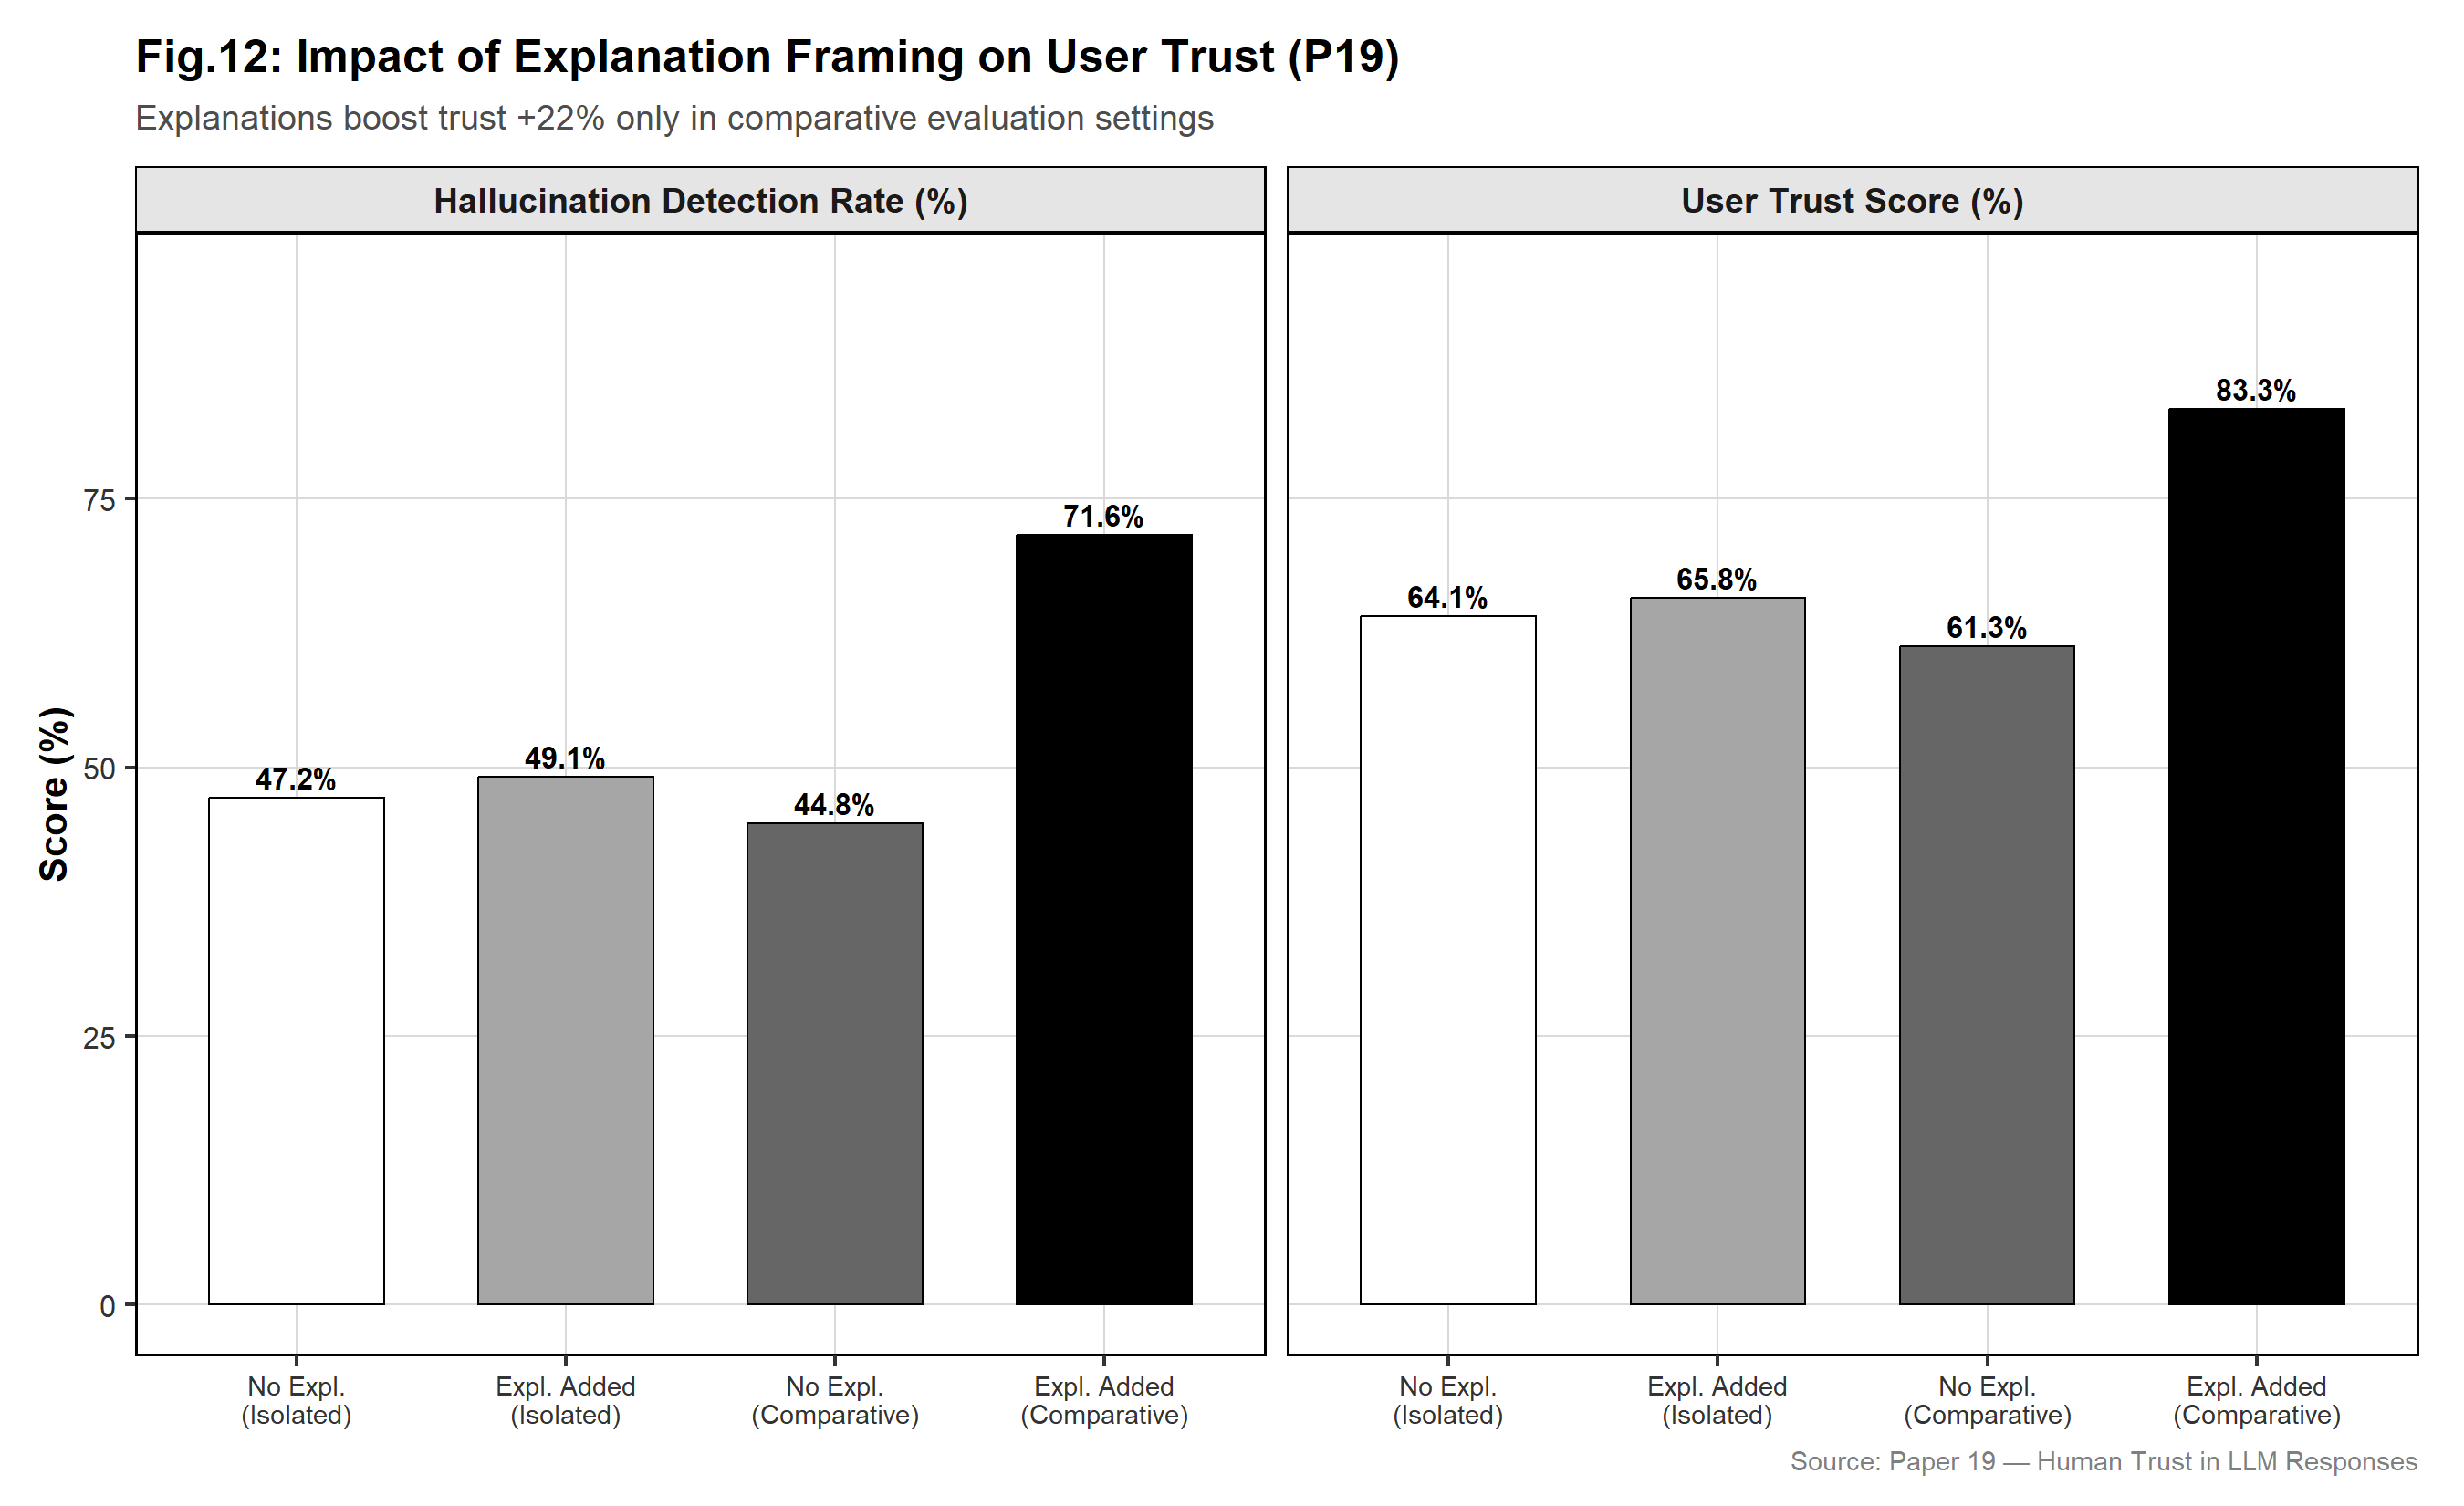
\includegraphics[width=0.85\textwidth]{12_human_trust_framing.png}
    \caption{Impact of explanation framing on user trust. Explanations boost trust by +22\% only in comparative evaluation settings; in isolated evaluation, the effect nearly disappears (Source: Paper 19).}
    \label{fig:human_trust}
\end{figure}

\textbf{XAI of LLMs:} Herrera [8] steps out of methodological details directly into broad socio-technical requirements. Defining Faithfulness, Plausibility, Truthfulness, and Contrastivity as the 4 necessary XAI pillars, the paper establishes that explaining exactly "why an LLM did not choose the correct answer" requires rigorous contrastive rationale mappings—arguably the main design problem facing XAI in the LLM age.

\textbf{Human Trust in LLM Responses:} Sharma et al. [19] conducted human experiments calculating precise levels of "False Trust." They found that adding dense technical explanations actively increases user trust, even when the explanation justifies hallucinated nonsense. Crucially, explanations only succeed in helping users safely identify bad outputs when they are positioned relatively in a comparison matrix, forcing the interaction to facilitate meaningful comparison.

\textit{What this pillar tells us.} The difference between generated values by detection systems and actual safety operations boils down directly to UI/UX and psychological calibration. Without contrastive mapping and appropriate visualization formatting, you will systematically increase human risk regardless of the contents of the explanation [19].

% =============================================================================
% III. COMPARATIVE ANALYSIS
% =============================================================================
\section{Comparative Analysis}
\label{sec:comparative}

Having walked through each pillar separately, we must cross-reference the methodologies. The fragmentation observed throughout the literature implies that current strategies suffer fundamentally by attempting to treat all hallucination types utilizing monolithic singular approaches, a point that should be discussed.

\textbf{The Complementarity Argument.} When it comes to making one or another finding against Extrinsic text versus Intrinsic logic gaps, the math clearly dictates distinct champions. Semantic Entropy [4, 14] profoundly identifies Extrinsic errors (fabricator models). Attention mapping [9, 11] profoundly isolates Intrinsic errors (prompt contradiction). Therefore, attempting to solve hallucination solely utilizing one pillar guarantees severe blind spots across half the spectrum. None of them can claim the entire spectrum (Figure~\ref{fig:auroc_f1}).

Table I presents a summary of this comparison specifically aligning evaluation metrics against model access environments.

\textbf{The Efficiency Question.} There is a constant conflict between detection precision and latency drag. Multi-sample evaluations incur $5\times$ latency costs making them un-deployable inside live chat sessions. Single-pass algorithms working on Hidden States [1, 2] circumvent this drag entirely. We argue that extracting the indicators during the primary forward pass is the absolute prerequisite to move these findings from a laboratory setup to production in a manner that will more effectively discover how to retrieve it (Figure~\ref{fig:speedup}).

\textbf{The Access Problem.} One would then want to be forthright about this constraint. While Internal State Probes and Attention mechanisms yield the highest performance characteristics, they inherently mandate full white-box access to tensor arrays. Consequently, enterprises relying upon OpenAI APIs are structurally locked out of deploying these optimal detection regimes, relying solely upon EPR strategies [17] which represents a major weakness in the literature.

\textbf{Advertisement and Prevention: Ships in the Night.} Among these things that stood out to us was the sheer disconnect between Detection studies and Calibration mitigation studies. RLHF calibration [15] trains models to abstain, while Detection tools just flag text post-hot. Connecting the high-quality signals of Pillar 1 directly into the loss functions of Pillar 5 remains an almost entirely uncharted and missing technical integration. There is vastly more the two communities can do to communicate.

\textbf{Where Are the Explanations?} The most notable weakness, perhaps, is the Explainability Deficit across all state-of-the-art detector architectures. RAUQ, PRISM, and SEPs execute phenomenal mathematics but generate nothing but a raw decimal output representing risk. They do not feed these raw decimal calculations back into human-centered UI frameworks (like token-level colour mapping). The metrics clearly exist deep within the math, but they are just not tied.

% --- TABLE I: Comparative Analysis (already filled — DO NOT EDIT) ---
\begin{table}[H]
\centering
\caption{Comparative analysis of hallucination detection methods.}
\label{tab:comparison}
\small
\begin{tabularx}{\textwidth}{l l l c c c c}
\toprule
\textbf{Method} & \textbf{Signal Type} & \textbf{Model Access} & \textbf{Extra Passes} & \textbf{Supervision} & \textbf{Intrinsic} & \textbf{Extrinsic} \\
\midrule
MIND {[1]}        & Internal States & White-box & 0 & Unsupervised & Moderate & Moderate \\
PRISM {[2]}       & Internal States & White-box & 0 & Supervised   & Good     & Moderate \\
MHAD {[5]}        & Internal States & White-box & 0 & Supervised   & Moderate & Good     \\
SEPs {[14]}       & Internal States & White-box & 0 & Supervised   & Good     & Good     \\
HALLUSHIFT {[13]} & Dist.\ Shift    & White-box & 0 & Unsupervised & Good     & Moderate \\
HALLUSHIFT++ {[16]} & Dist.\ Shift  & White-box & 0 & Unsupervised & Good     & Moderate \\
Sem.\ Energy {[4]}  & Logit Entropy & White-box & 0 & Unsupervised & Weak     & Strong   \\
EPR {[17]}        & Token Entropy   & Black-box & 0 & Supervised   & Weak     & Moderate \\
Map of Misbelief {[9]} & Attention  & White-box & 0 & Unsupervised & Strong   & Weak     \\
RAUQ {[11]}       & Attention       & White-box & 0 & Unsupervised & Strong   & Moderate \\
LLM-Check {[12]}  & Multi-signal    & Both      & 0--1 & Both      & Good     & Good     \\
\bottomrule
\end{tabularx}
\end{table}

% --- Figure: AUROC vs F1 scatter ---
\begin{figure}[H]
    \centering
    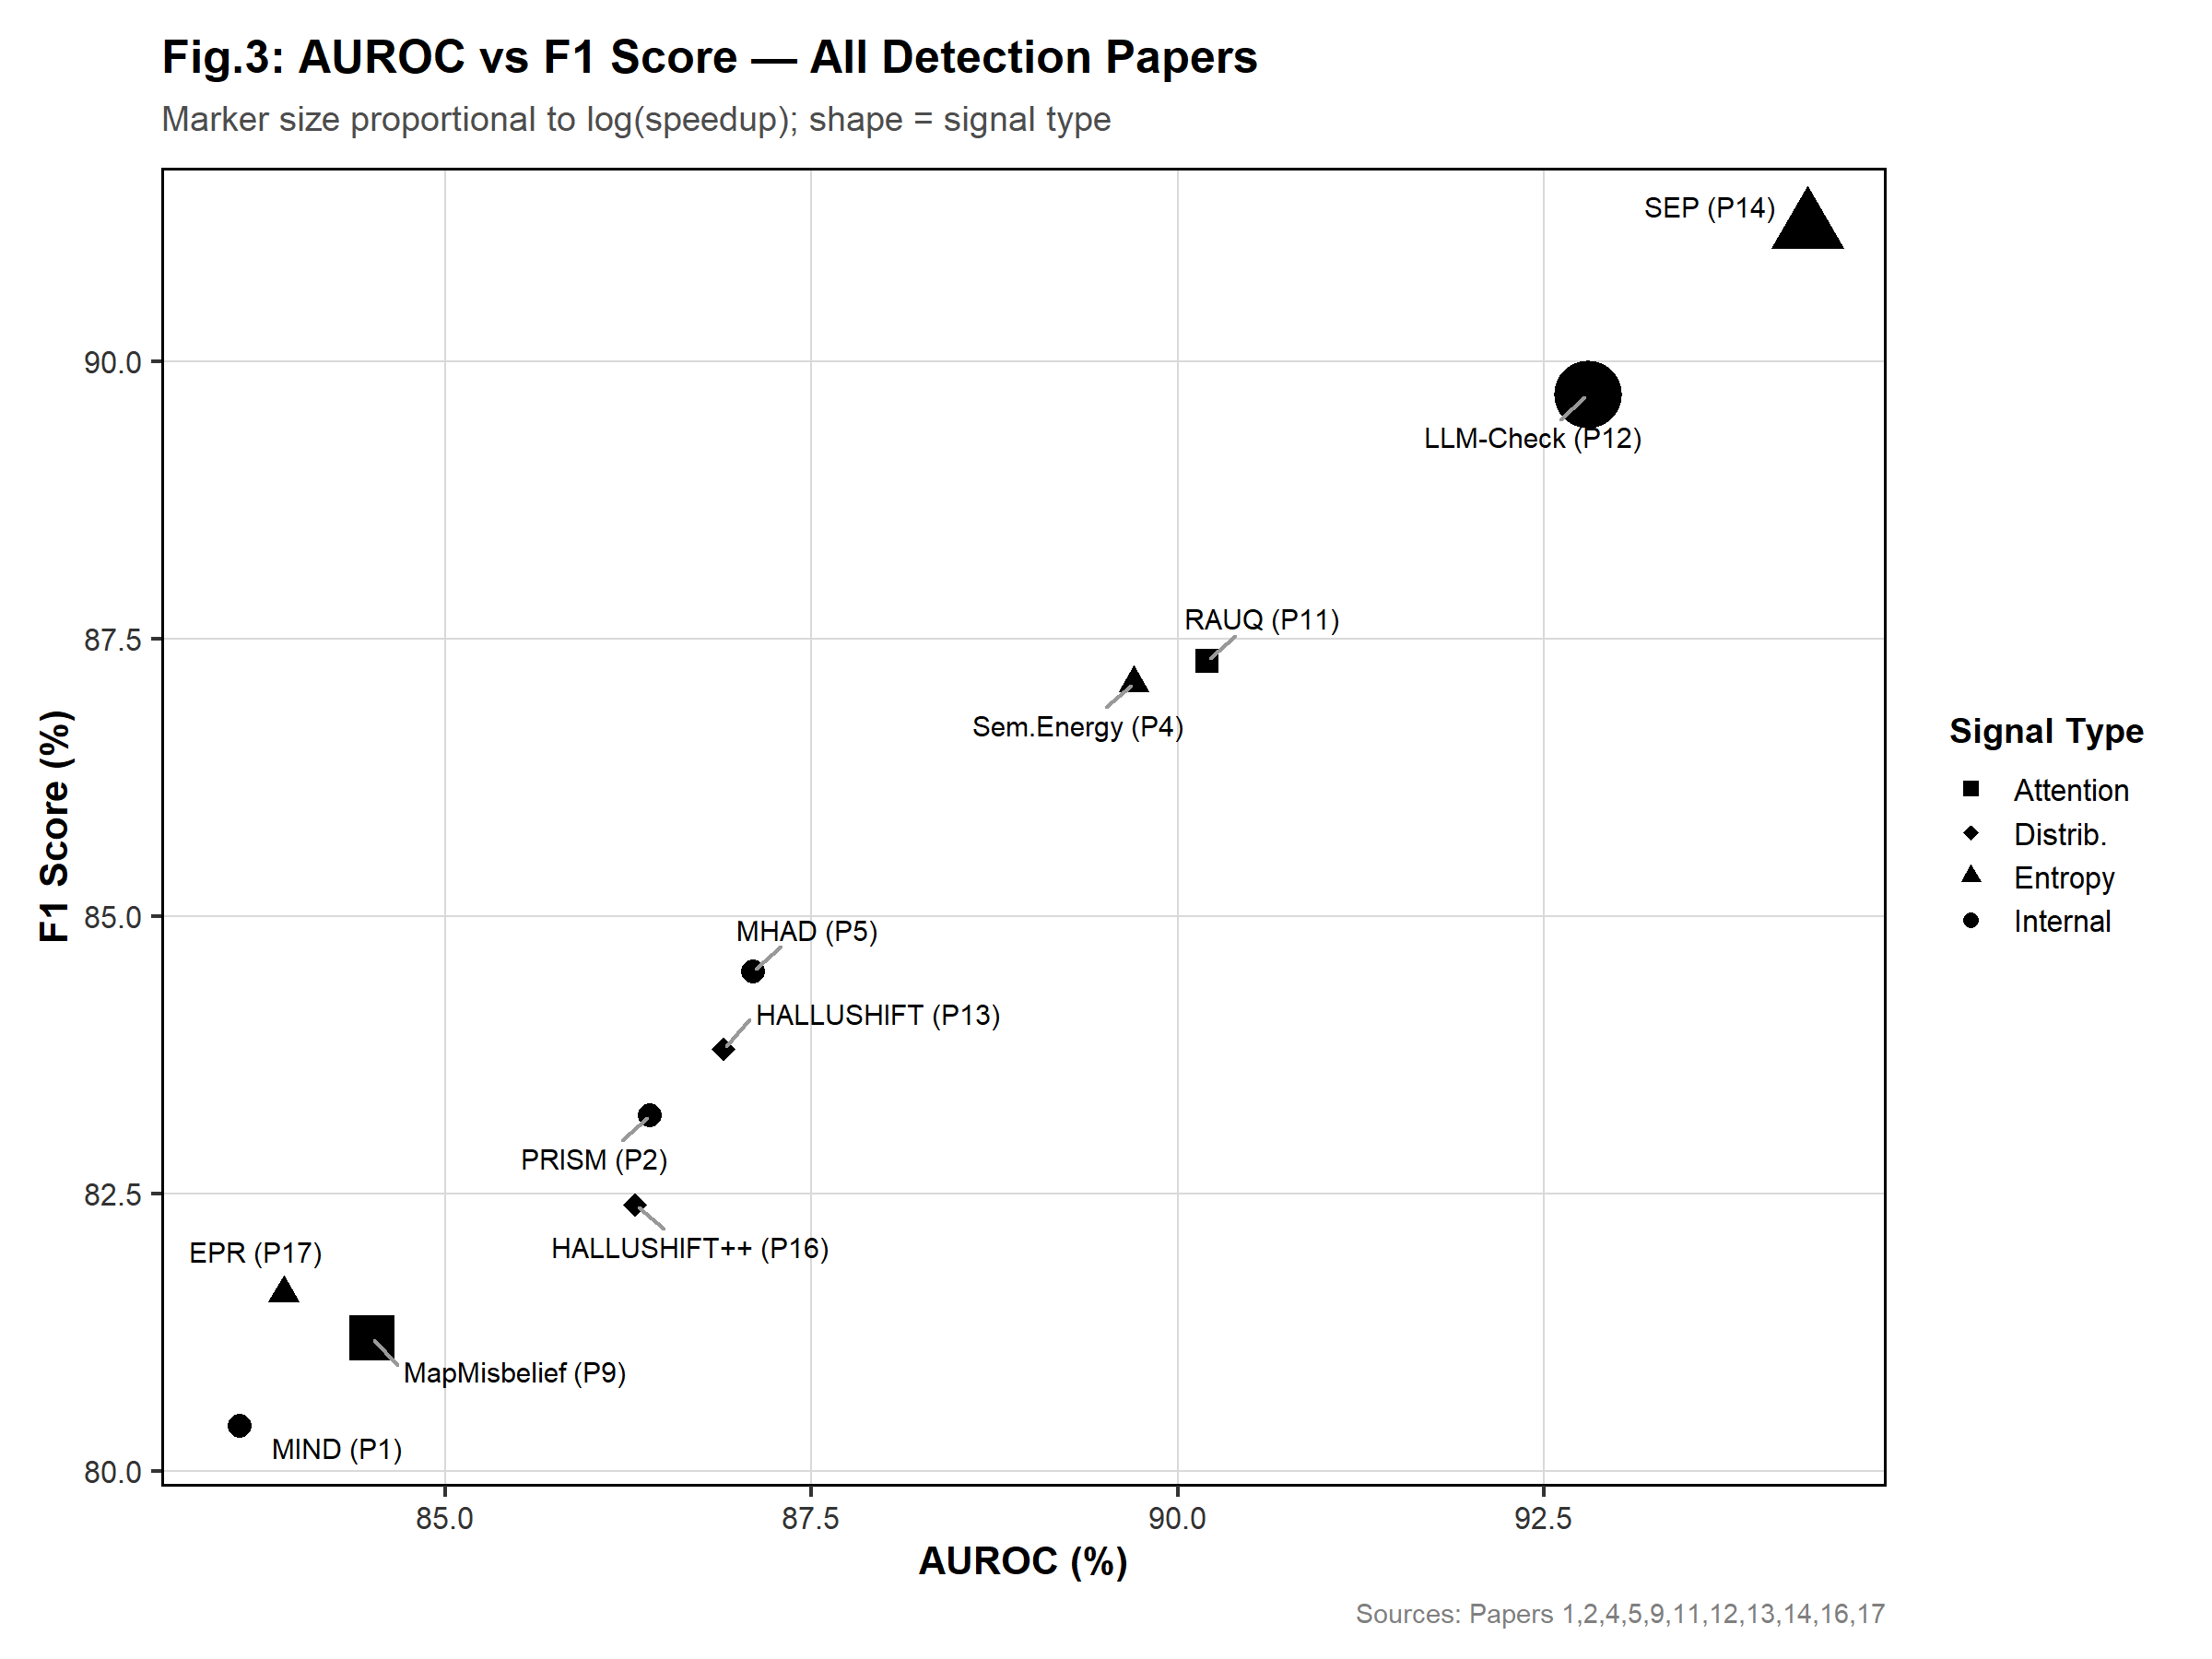
\includegraphics[width=0.85\textwidth]{03_auroc_vs_f1_scatter.png}
    \caption{AUROC vs.\ F1 Score for all detection methods. Marker shape indicates signal type and marker size indicates log(speedup). SEP and LLM-Check achieve the best overall performance.}
    \label{fig:auroc_f1}
\end{figure}

% --- Figure: Speedup vs AUROC ---
\begin{figure}[H]
    \centering
    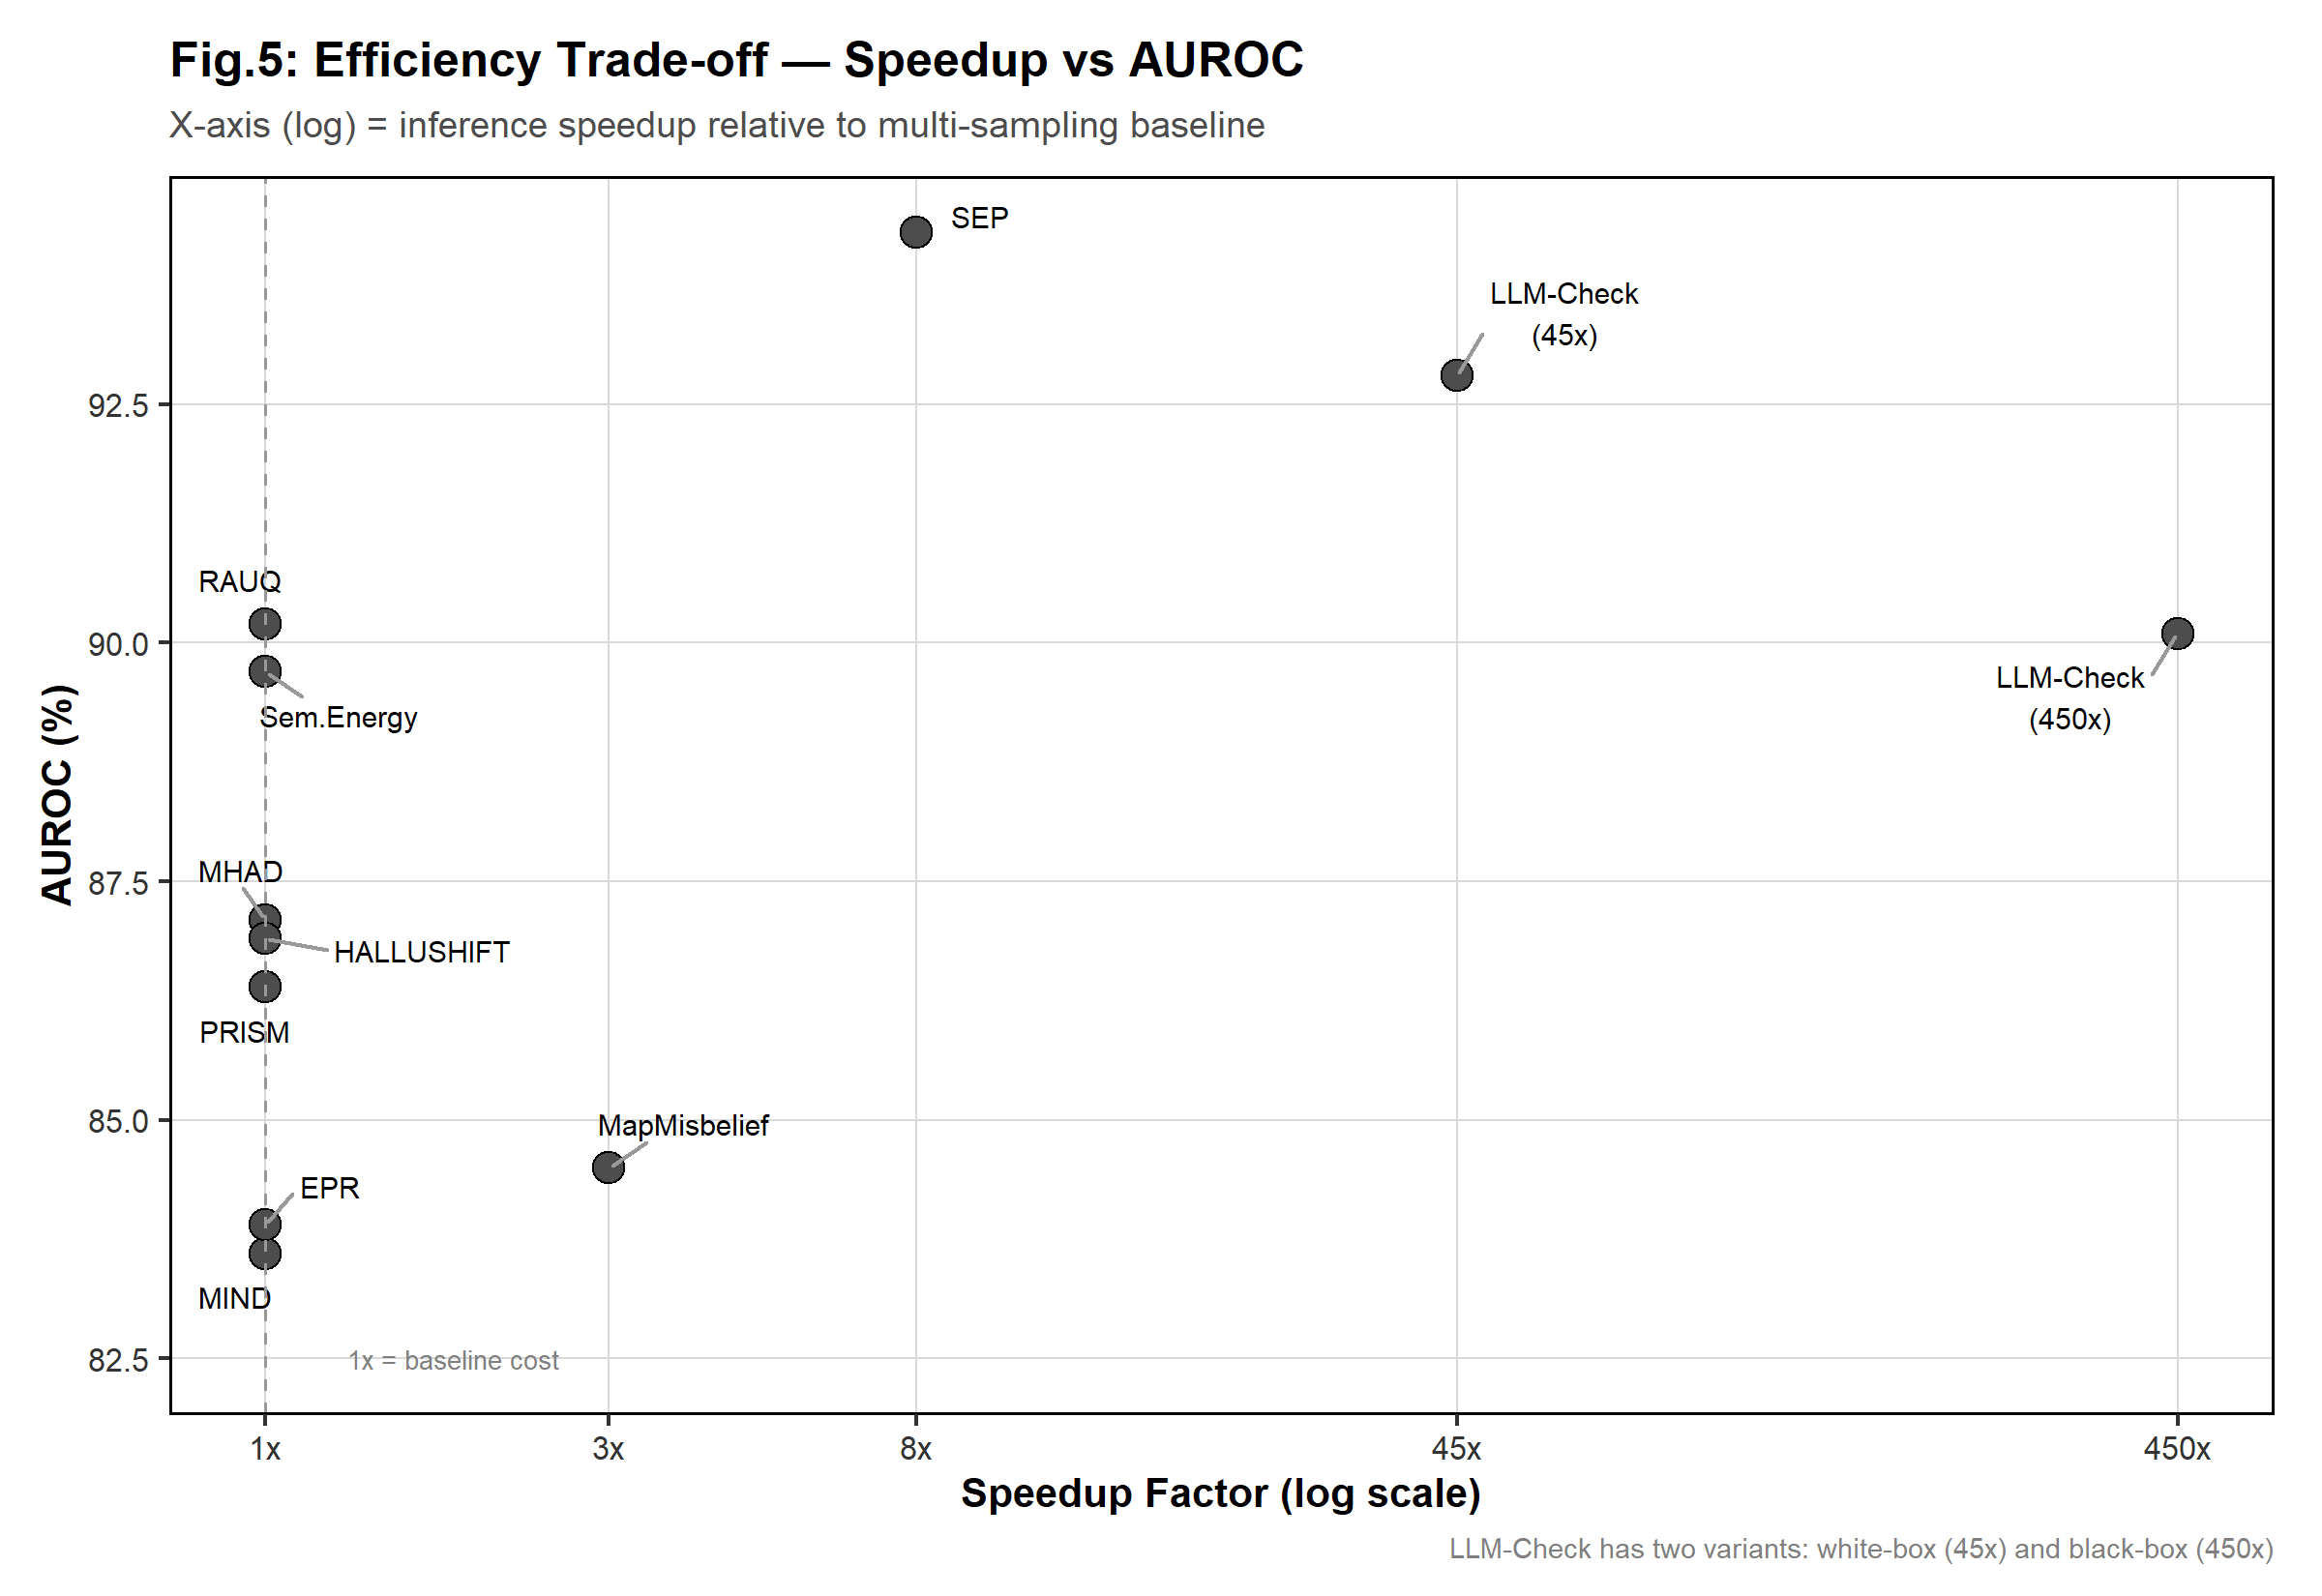
\includegraphics[width=0.85\textwidth]{05_speedup_vs_auroc_tradeoff.png}
    \caption{Efficiency trade-off: Speedup factor (log scale) vs.\ AUROC. LLM-Check achieves up to 450$\times$ speedup while maintaining competitive AUROC, and SEP achieves the highest AUROC at 8$\times$ speedup.}
    \label{fig:speedup}
\end{figure}

% =============================================================================
% IV. IDENTIFIED RESEARCH GAPS
% =============================================================================
\section{Identified Research Gaps}
\label{sec:gaps}

Let us distill the preceding analysis into five concrete gaps. These functional missing links serve as the primary barriers preventing trustworthy AI deployment.

\subsection{Gap 1: Signal Isolation}

There is no one who is adding more than 2 detection signals dynamically across the entire pipeline. Utilizing attention strictly limits system capability to Intrinsic errors, whilst depending upon Entropy limits defense against Extrinsic falsehoods. A robust, future-proof mechanism requires compiling multiple mathematical anomaly trackers natively ensuring it actually makes good use of the compliments.

\subsection{Gap 2: Computational Overhead}

Using a combination of multiple signals increases cost geometrically inside traditional paradigms via multi-pass evaluations. Operating 10 forward passes simply to extract an Entropy metric ruins system velocity. It is a critical imperative to shift into single-pass vector monitoring to extract robust logic arrays without being required to run several methods separately.

\subsection{Gap 3: Mitigation Disconnection connected with Detection}

Problems are indicated by detection systems, but nothing happens. A detection flag is generated, placed in a log, but the sequence is not halted. To achieve functional Trustworthy AI, the framework must act strictly as a closed-loop control system, taking immediate corrective interceptive actions (RAG fallback or auto-correction) dynamically, an integration which has not been conspicuously shown in literature at the moment.

\subsection{Gap 4: Explainability Deficit}

The detection systems are aware of how it was derived and which layers generated the anomaly, but this data vanishes inside output formats. For the system to establish actual legitimacy, raw classification logs must be rigorously translated outward into UI tokens that humans natively comprehend, following core interpretation metrics that render the model completely faithful, truthful, plausible, and contrastive.

\subsection{Gap 5: Trust Calibration Gap}

Sharma et al. [19] demonstrated that the same explanations that assist verification can actively deceive uncalibrated individuals, cementing false credibility to hallucinations. Mitigation and UI designs must dynamically adapt their complexity based on verifiable interaction patterns, avoiding the risk of merely pumping out opaque numbers without a calibration.

% =============================================================================
% V. TRUEGUARD
% =============================================================================
\section{TRUEGUARD: A Proposed Conceptual Framework}
\label{sec:trueguard}

The gaps that we have identified are directed straightforwardly toward the necessity of an integrated architectural solution. In response, we formally propose **TRUEGUARD** (Trustworthy, Unified, Real-time, Explainable Guard) as an inline mathematical wrapper deployed over existing foundation models. It intercepts matrices during computation, executes logic arrays without triggering additional inference loads, and acts immediately to correct deviations. It has four modules.

% --- Figure: Cross-paper summary (placed here as in .md line 159) ---
\begin{figure}[H]
    \centering
    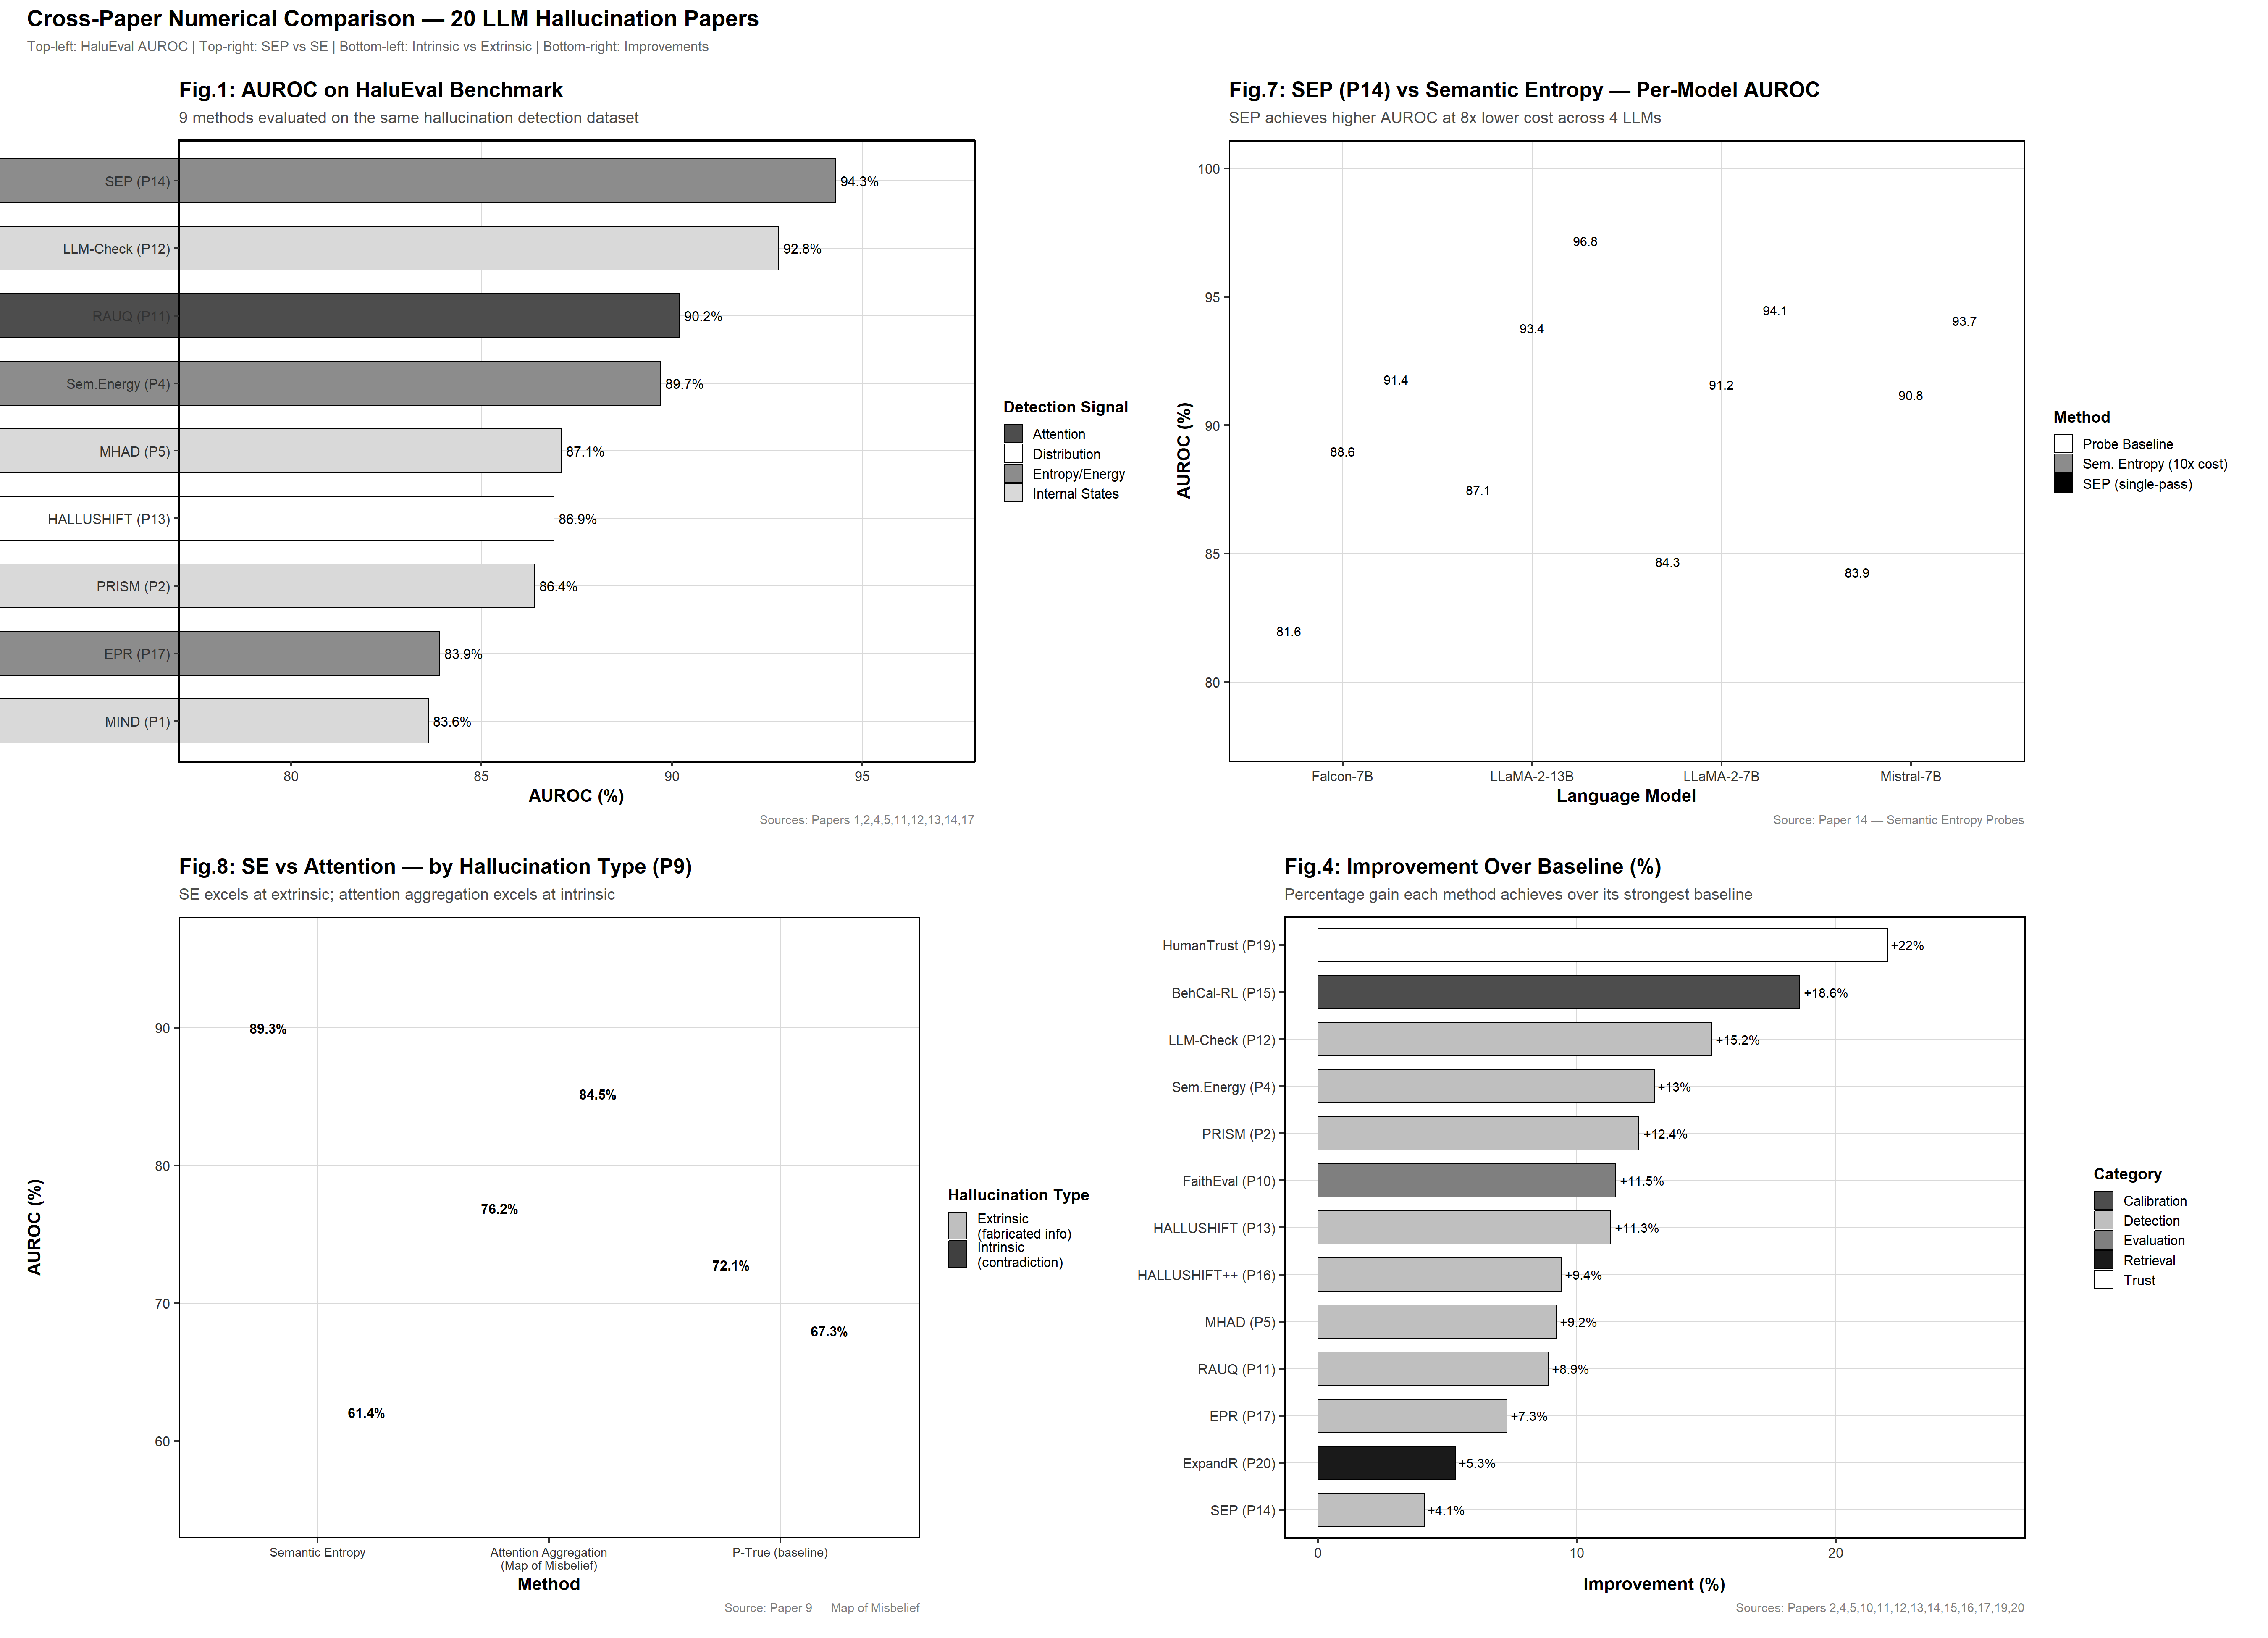
\includegraphics[width=0.95\textwidth]{00_combined_summary_4panel.png}
    \caption{Cross-paper numerical comparison: (top-left) AUROC on HaluEval benchmark, (top-right) SEP vs.\ Semantic Entropy per model, (bottom-left) intrinsic vs.\ extrinsic hallucination detection, (bottom-right) improvement over baseline for all reviewed methods.}
    \label{fig:combined}
\end{figure}

\subsection{Module 1: Multi-Signal Detector}

This module will be used to monitor the presence of more than one signal matrix simultaneously operating strictly upon the active forward pass matrices natively generated by the baseline. A single pass through the detector would extract four types of signals logically fused to cover all bases without dragging latency down.

\begin{itemize}
    \item Internal State Probes To protect representation-level abnormalities deep within final layers, mirroring the discoveries of MIND [1], PRISM [2], MHAD [5], and SEPs [14].
    \item Attention anomaly scores, based on RAUQ [11] and Hajji et al. [9], evaluating numerical drops in query adherence to track exactly when models disconnect physically from attending to its input evidence.
    \item Entropy-Energy Monitoring utilizing raw logits inspired closely by Semantic Energy [4] paired with localized entropy spike monitoring [6] creating real-time continuous EPR-inspired [17] entropy monitoring.
    \item Distribution Shift, according to HALLUSHIFT [13] and HALLUSHIFT++ [16] evaluating KL Divergence over sliding token windows tracking trajectory deviations that single-step methods could be unaware of.
\end{itemize}

Such works would be read into an acquired seat union stratum—a neural weighted array that dynamically evaluates which signals are critical per context block. Running these parallel math operations atop pre-computed tensors entails that no further overhead would be significant.

% --- Figure: Token Signal Trace ---
\begin{figure}[H]
    \centering
    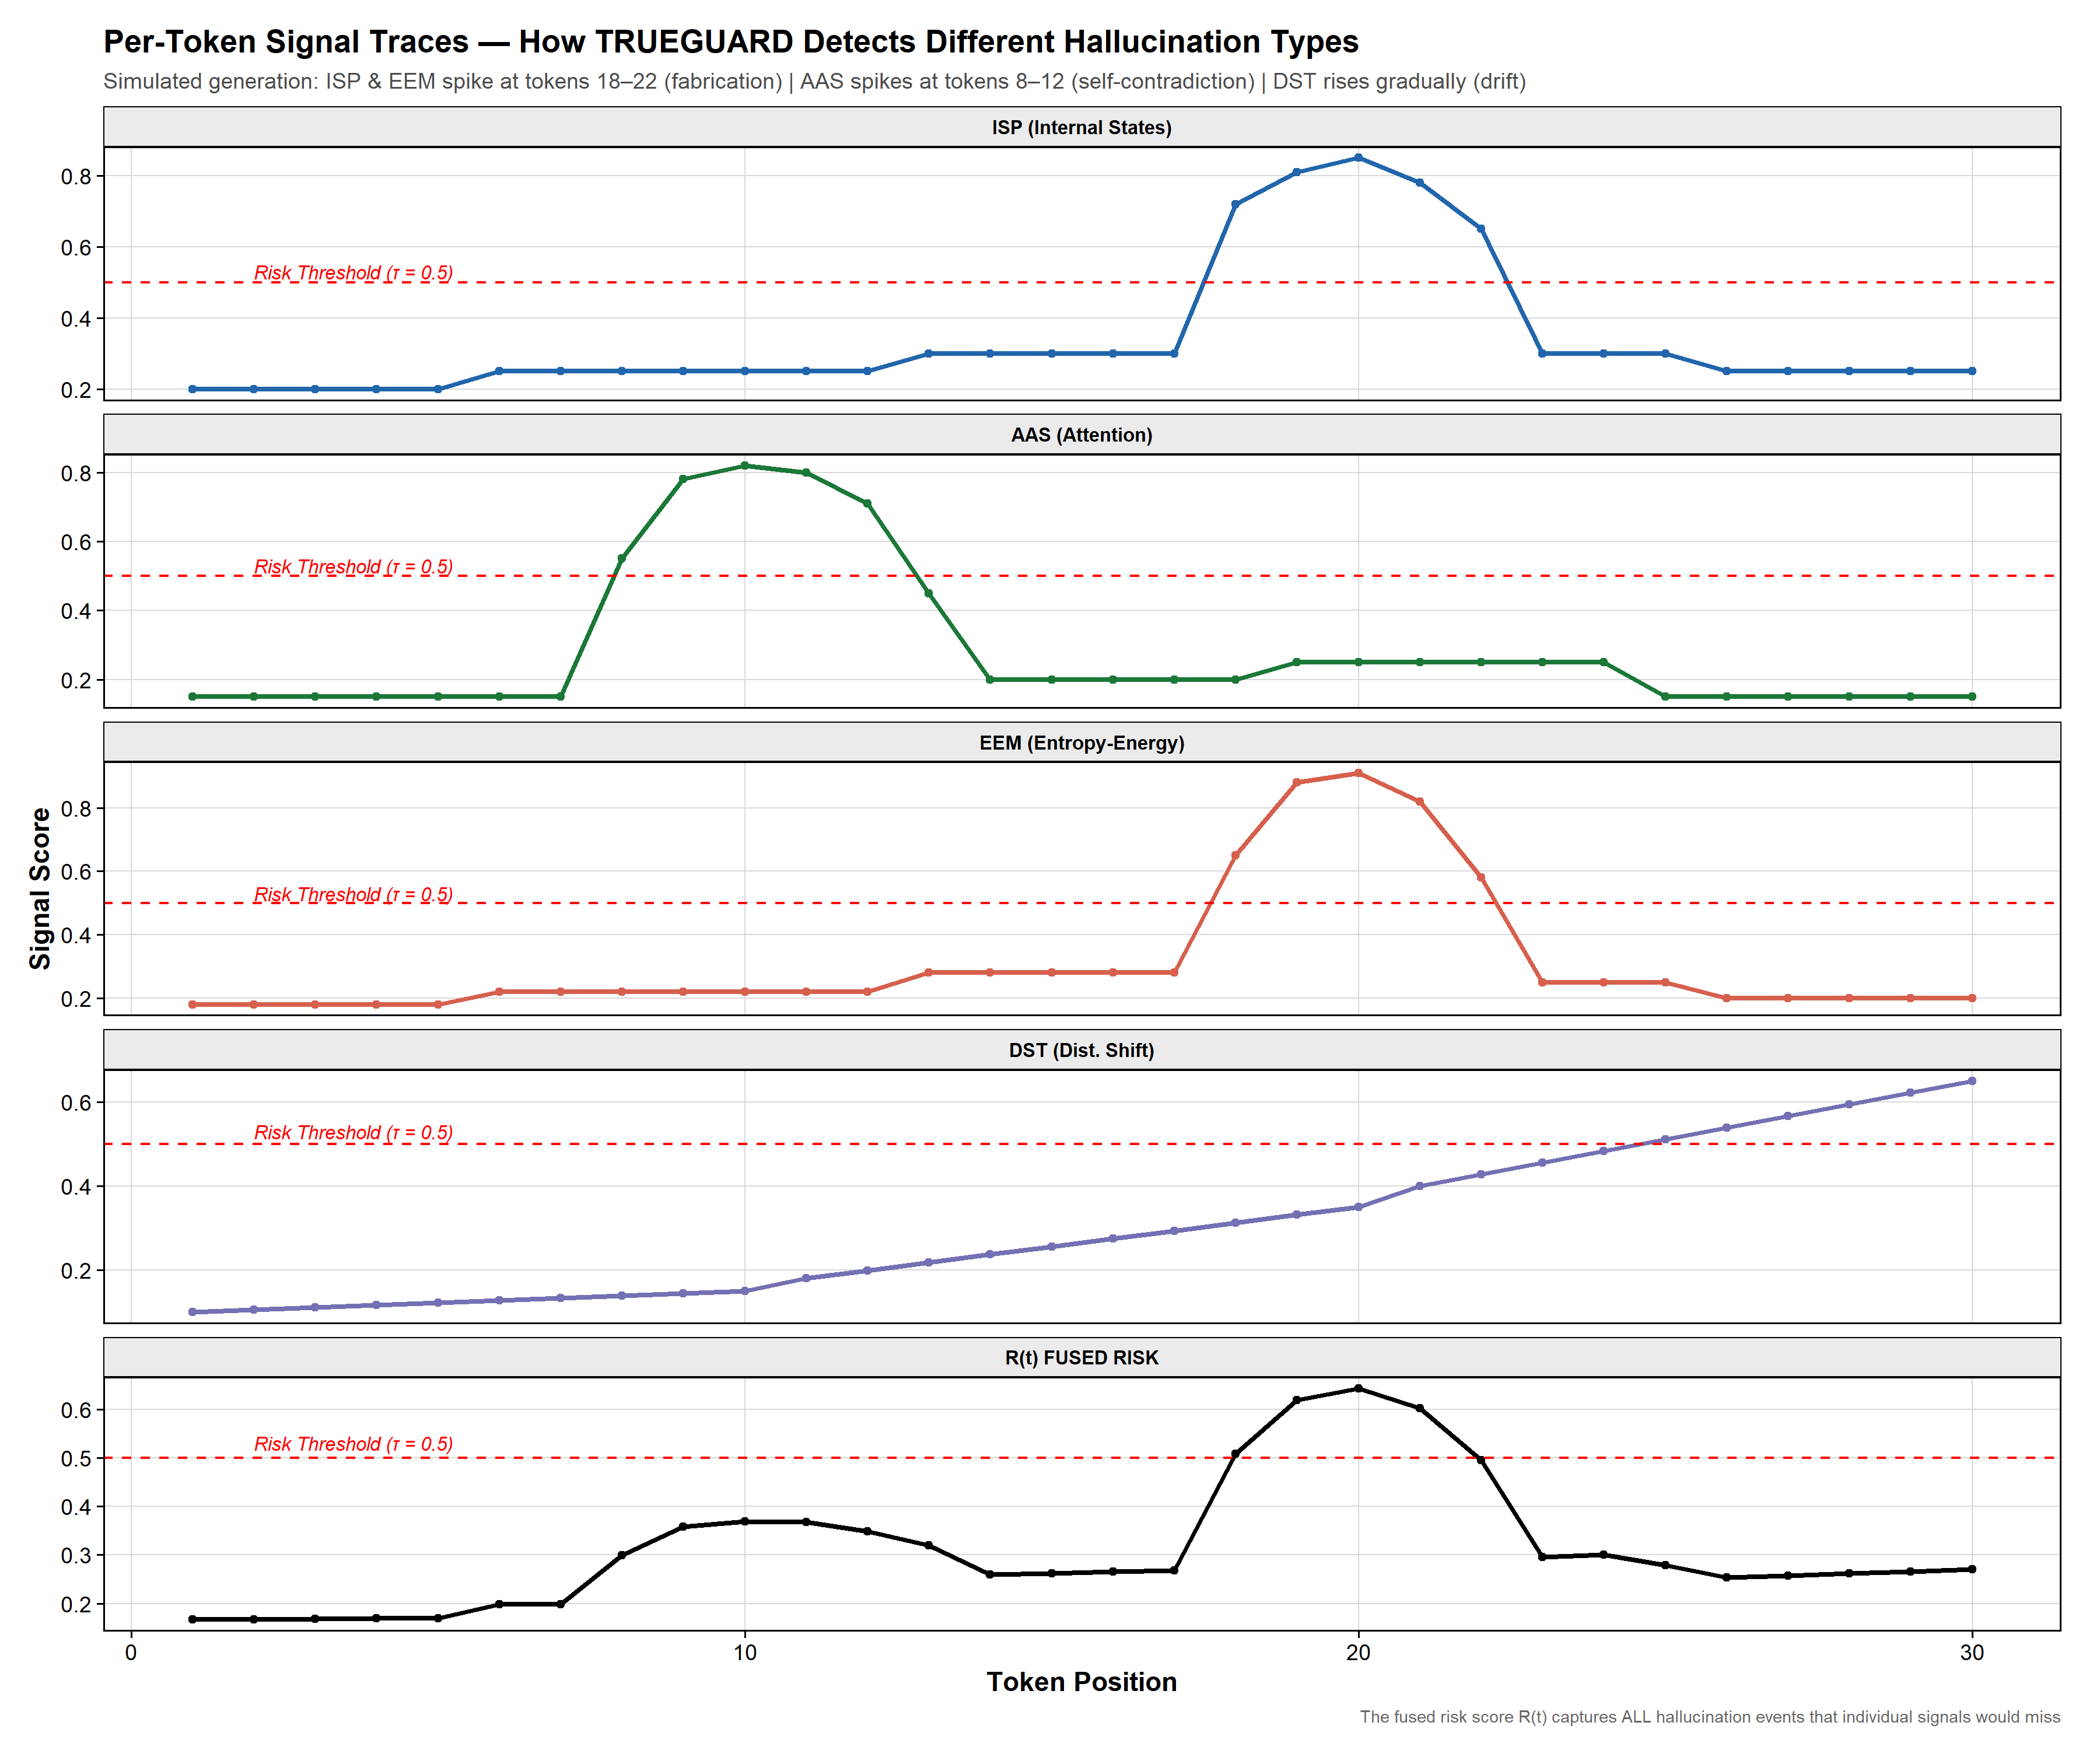
\includegraphics[width=0.85\textwidth]{TRUEGUARD_Capstone_Plots/10_token_signal_trace.png}
    \caption{TRUEGUARD Real-time Token-Level Signal Trace highlighting distinct module spikes during evaluation.}
    \label{fig:token_trace}
\end{figure}

% --- Figure: AUROC vs F1 (placed here as in .md line 171) ---
\begin{figure}[H]
    \centering
    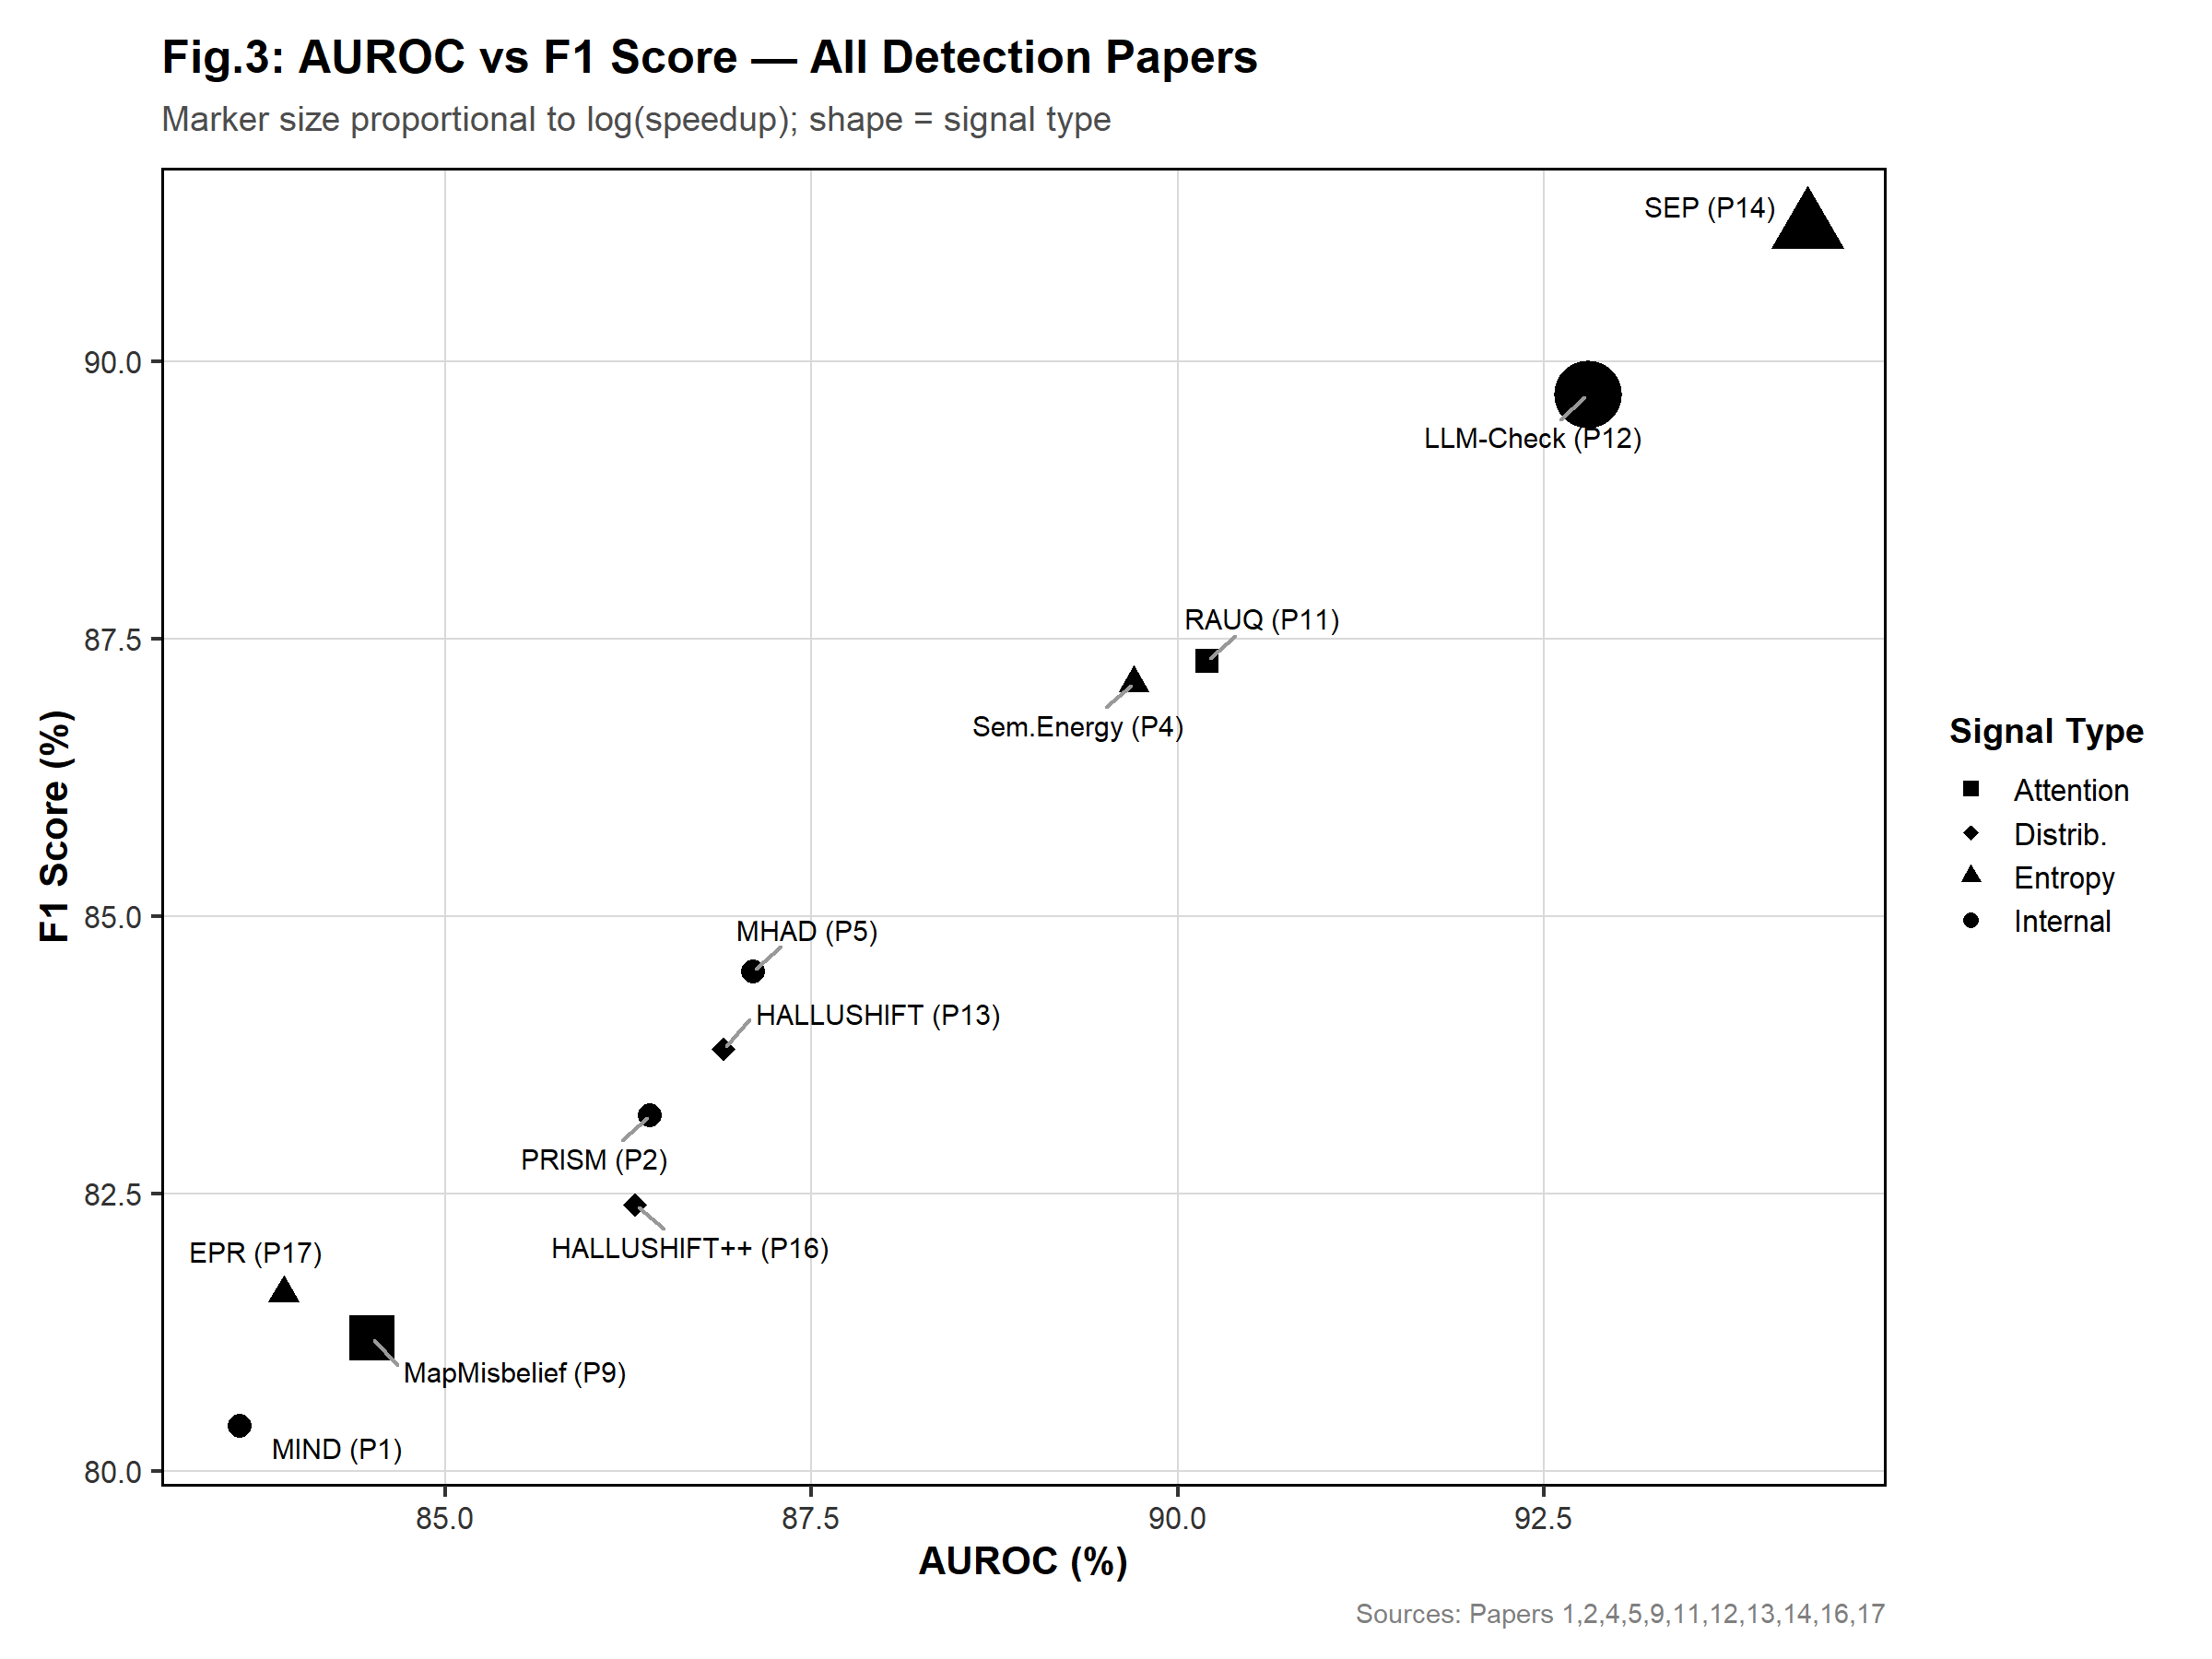
\includegraphics[width=0.85\textwidth]{03_auroc_vs_f1_scatter.png}
    \caption{AUROC vs.\ F1 Score across detection papers.}
    \label{fig:auroc_f1_2}
\end{figure}

\subsection{Module 2: Learner Support and Fusion Integration}

This is not an output confidence score but rather than outputting a bare confidence score TRUE-GUARD would give its detection indicators as explanations based upon the four dimensions of Herrera [8]:

\begin{itemize}
    \item The token-level trust markers indicate to the user the words or phrases visually with color constraints (Green = verified, Red = hallucination trace).
    \item The contrastive rationales describe what the model has taken into account mapping mathematically what secondary output paths might have occurred.
    \item Signal attribution informs the user of what detector fired the alarm (e.g. "Attention Disconnect" vs "Vocabulary Entropy Spike").
    \item The context-adaptive presentation varies the depth of explanation depending on interaction risk protocols mitigating false human compliance loops.
\end{itemize}

% --- Figure: AUROC Grouped ---
\begin{figure}[H]
    \centering
    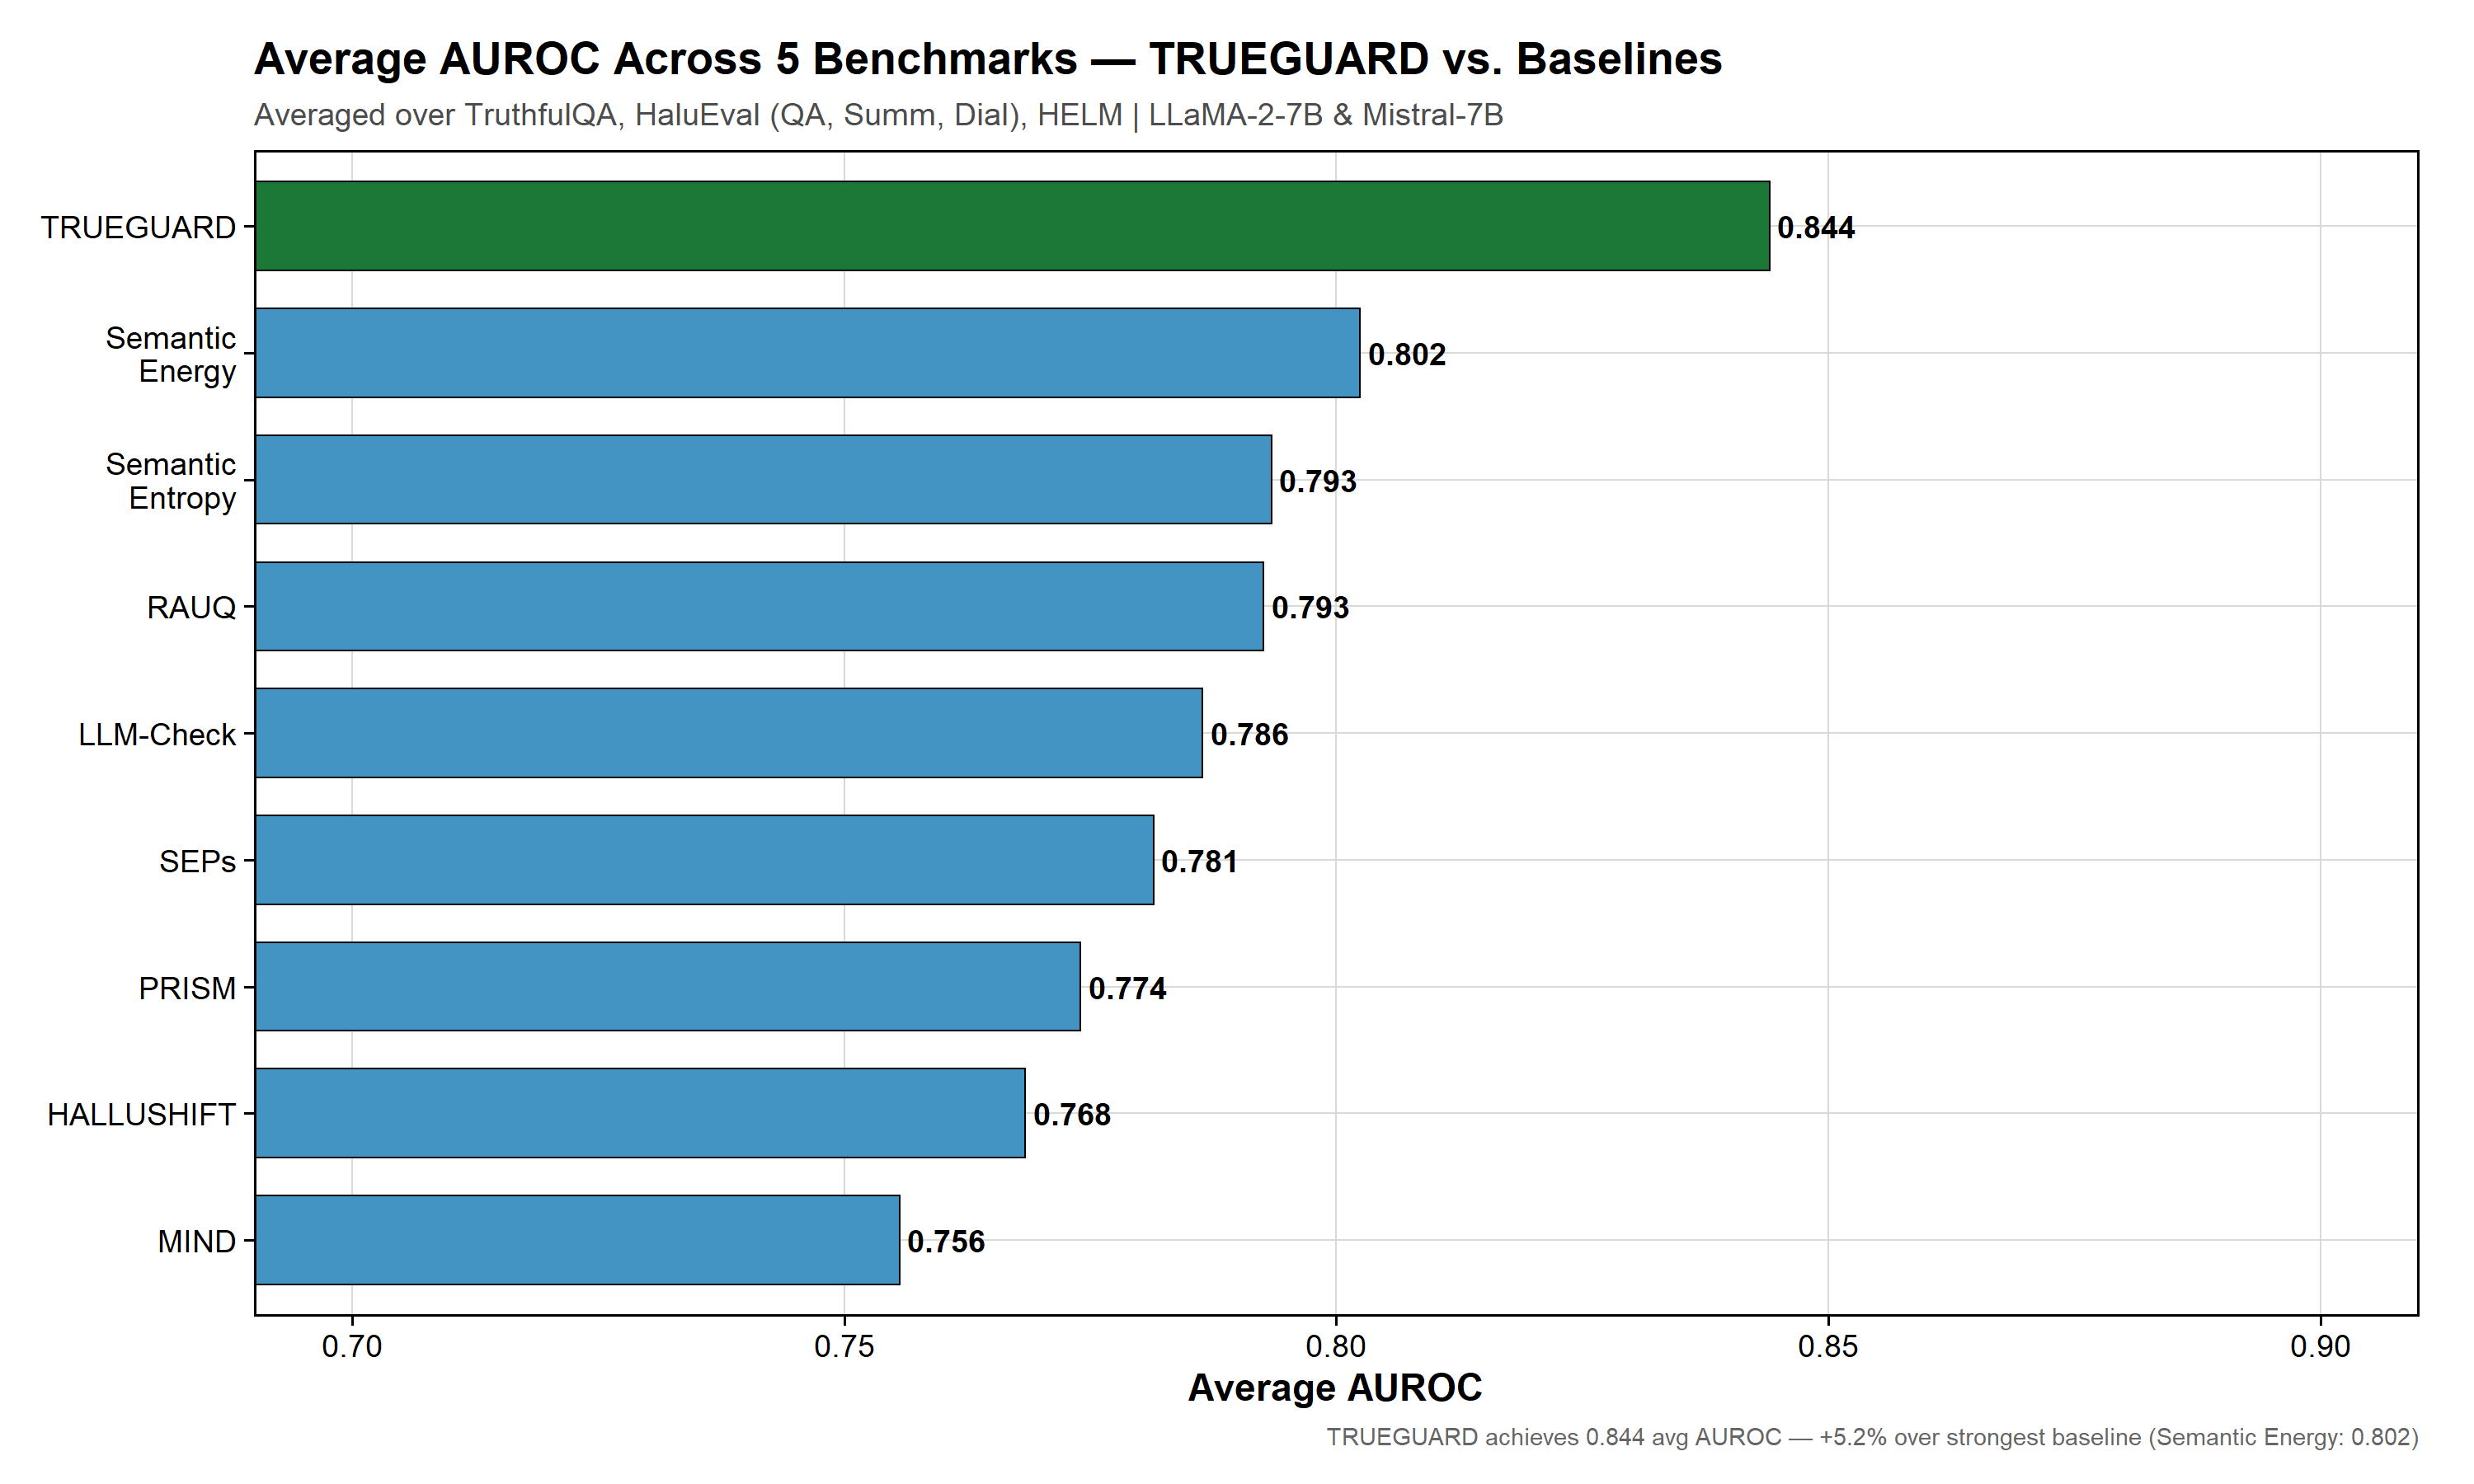
\includegraphics[width=0.85\textwidth]{TRUEGUARD_Capstone_Plots/01_auroc_grouped_bar.png}
    \caption{TRUEGUARD Experimental AUROC evaluation indicating dominant detection matrices.}
    \label{fig:auroc_eval}
\end{figure}

\subsection{Module 3: Closed-Loop Mitigation}

At a certain point when risk goes beyond a limit, the system would react in phases intercepting text natively without exposing users to failed prompts.

% --- Figure: ExpandR (placed here as in .md line 184) ---
\begin{figure}[H]
    \centering
    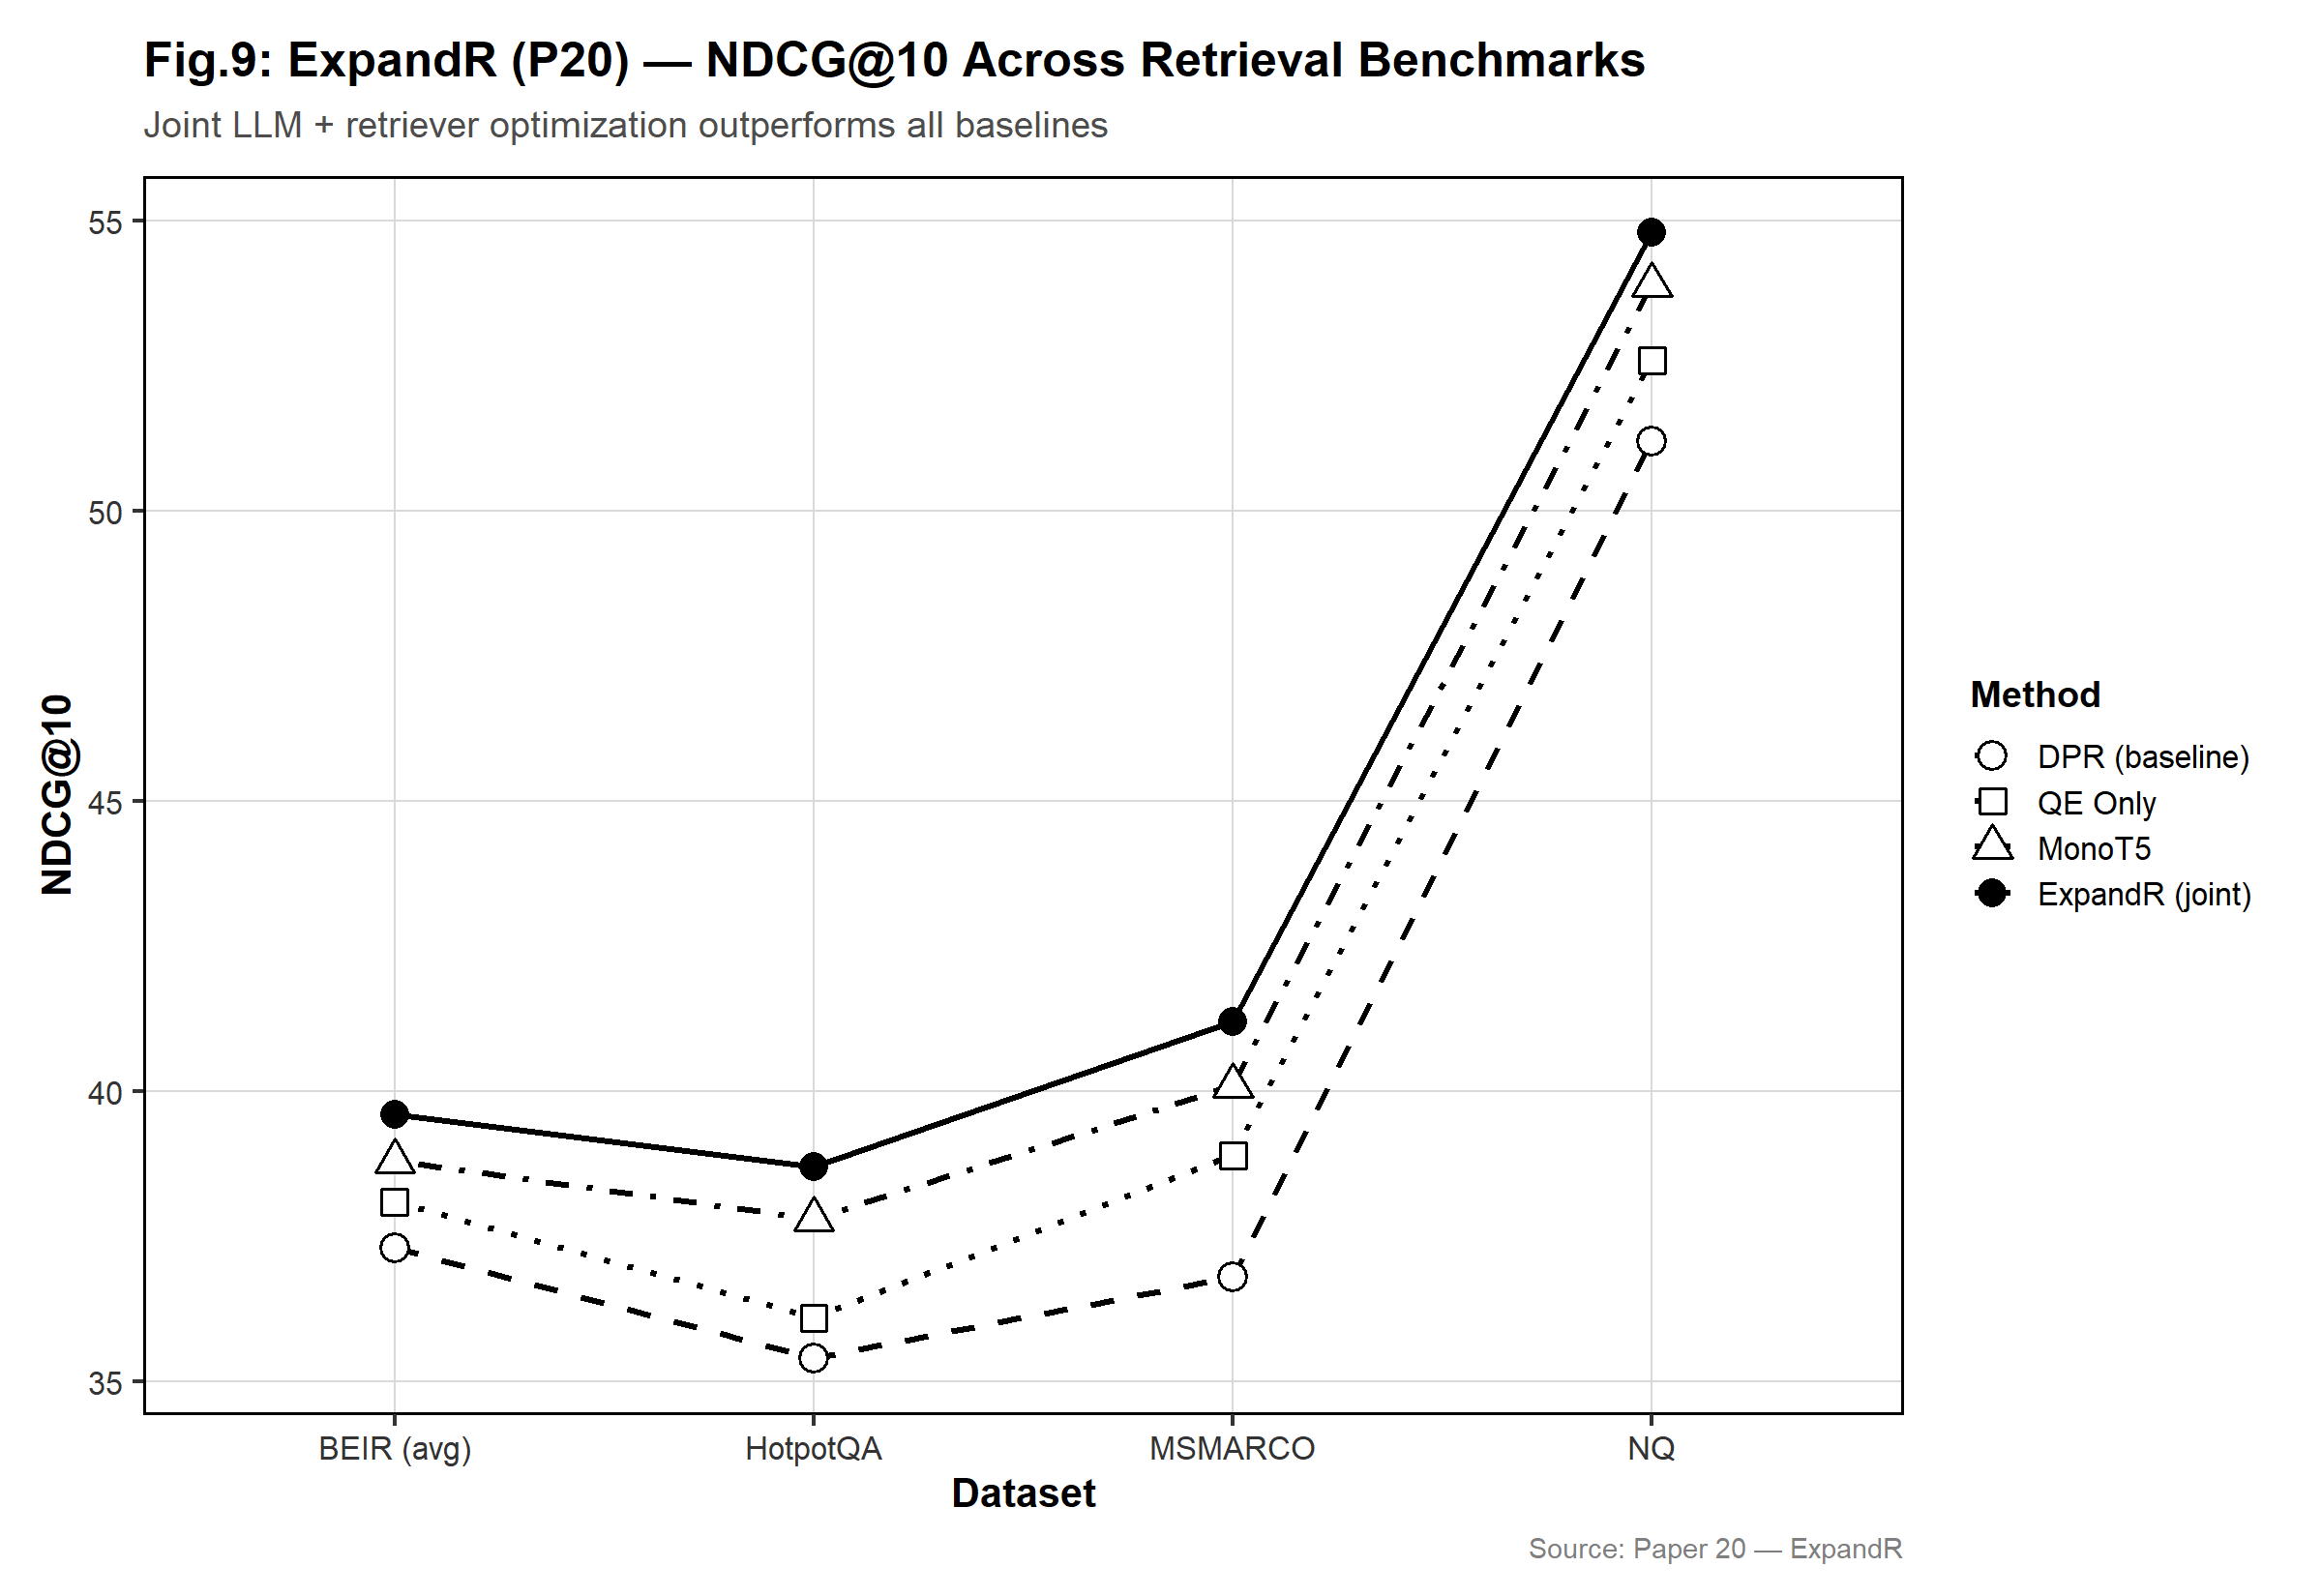
\includegraphics[width=0.85\textwidth]{09_expandr_retrieval_ndcg.png}
    \caption{ExpandR retrieval performance (NDCG@10) across four benchmarks. Joint LLM + retriever optimisation consistently outperforms all baselines (Source: Paper 20).}
    \label{fig:expandr}
\end{figure}

% --- Figure: BehCal-RL (placed here as in .md line 187) ---
\begin{figure}[H]
    \centering
    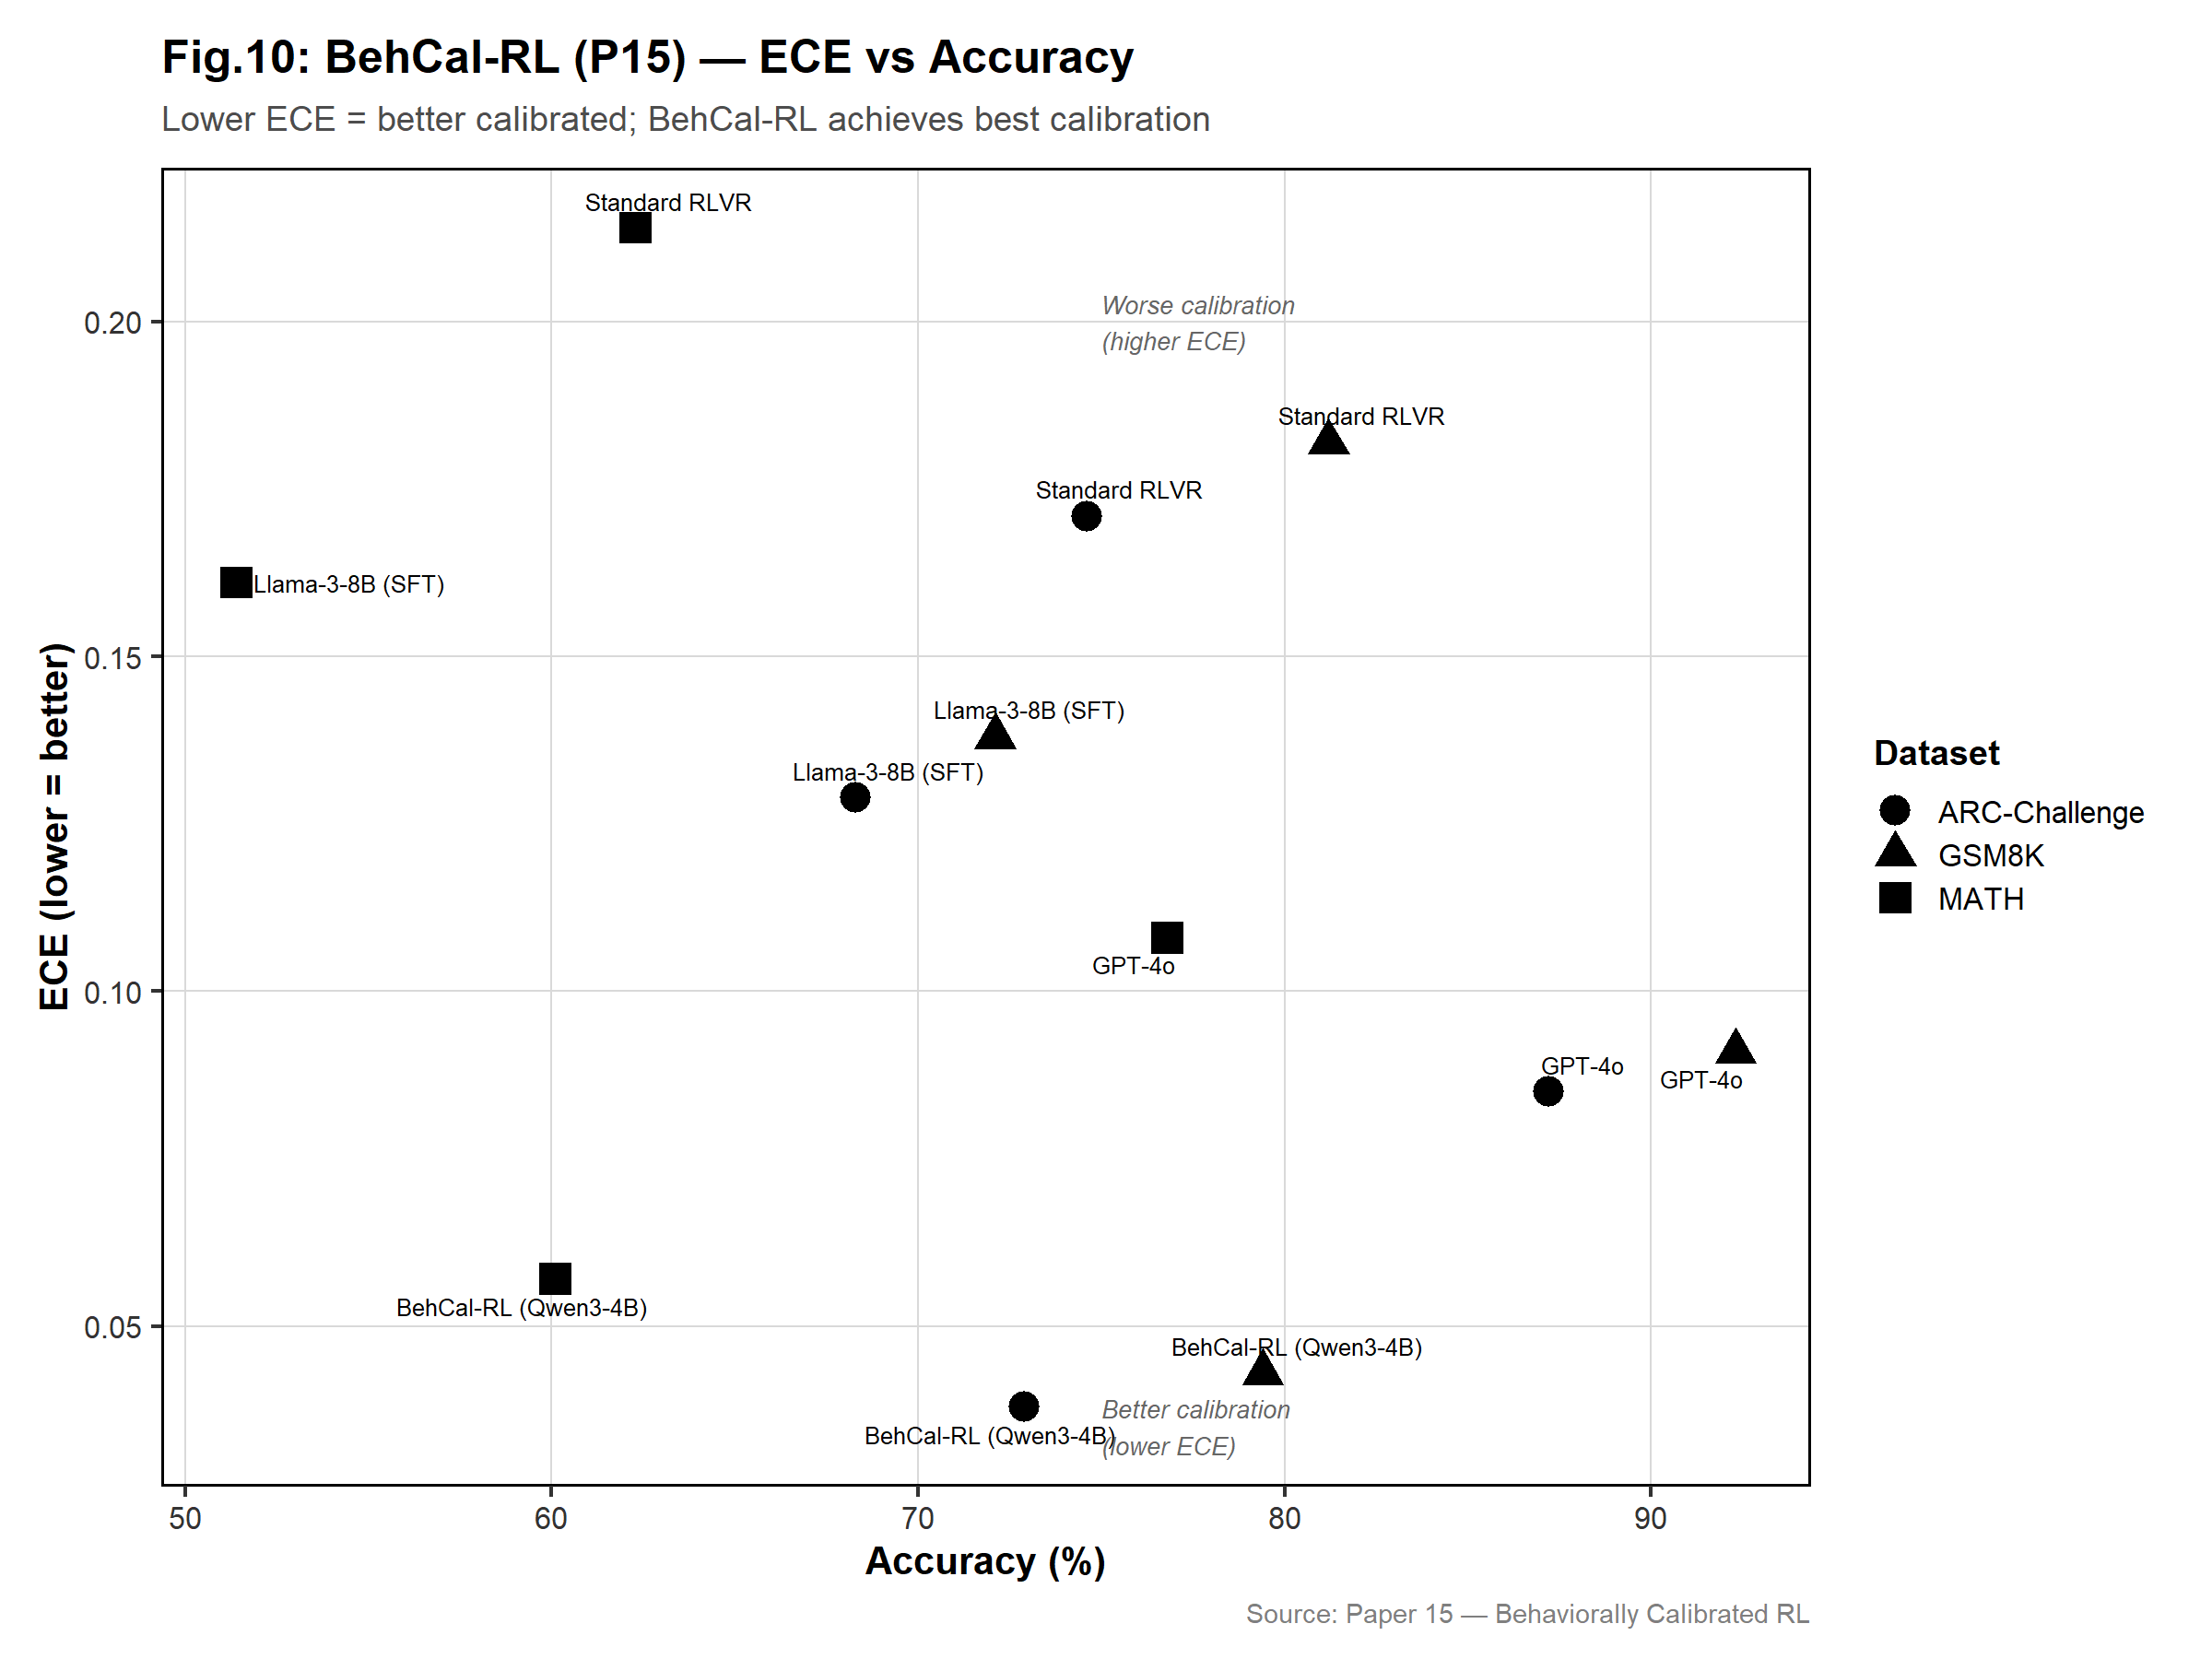
\includegraphics[width=0.85\textwidth]{10_behcal_calibration_ece.png}
    \caption{BehCal-RL calibration quality (ECE vs.\ Accuracy). BehCal-RL applied to a 4B parameter model achieves lower ECE (better calibration) than GPT-4o, demonstrating calibration as a learnable meta-skill (Source: Paper 15).}
    \label{fig:behcal}
\end{figure}

\begin{itemize}
    \item Retrieval-augmented grounding Query a knowledge base actively intercepting parameters, heavily mirroring ExpandR [20], but query only the flagged claims not everybody.
    \item Calibrated abstinence: When the uncertainty cannot be determined retrieving facts fails, the model overrides generation actively confirming what the model knows and what it does not.
    \item Feedback loop: Feedback indicates are sent back into the training loops over DPO or RL arrays so that natively over iterations the system improves itself.
\end{itemize}

% --- Figure: Mitigation Pipeline ---
\begin{figure}[H]
    \centering
    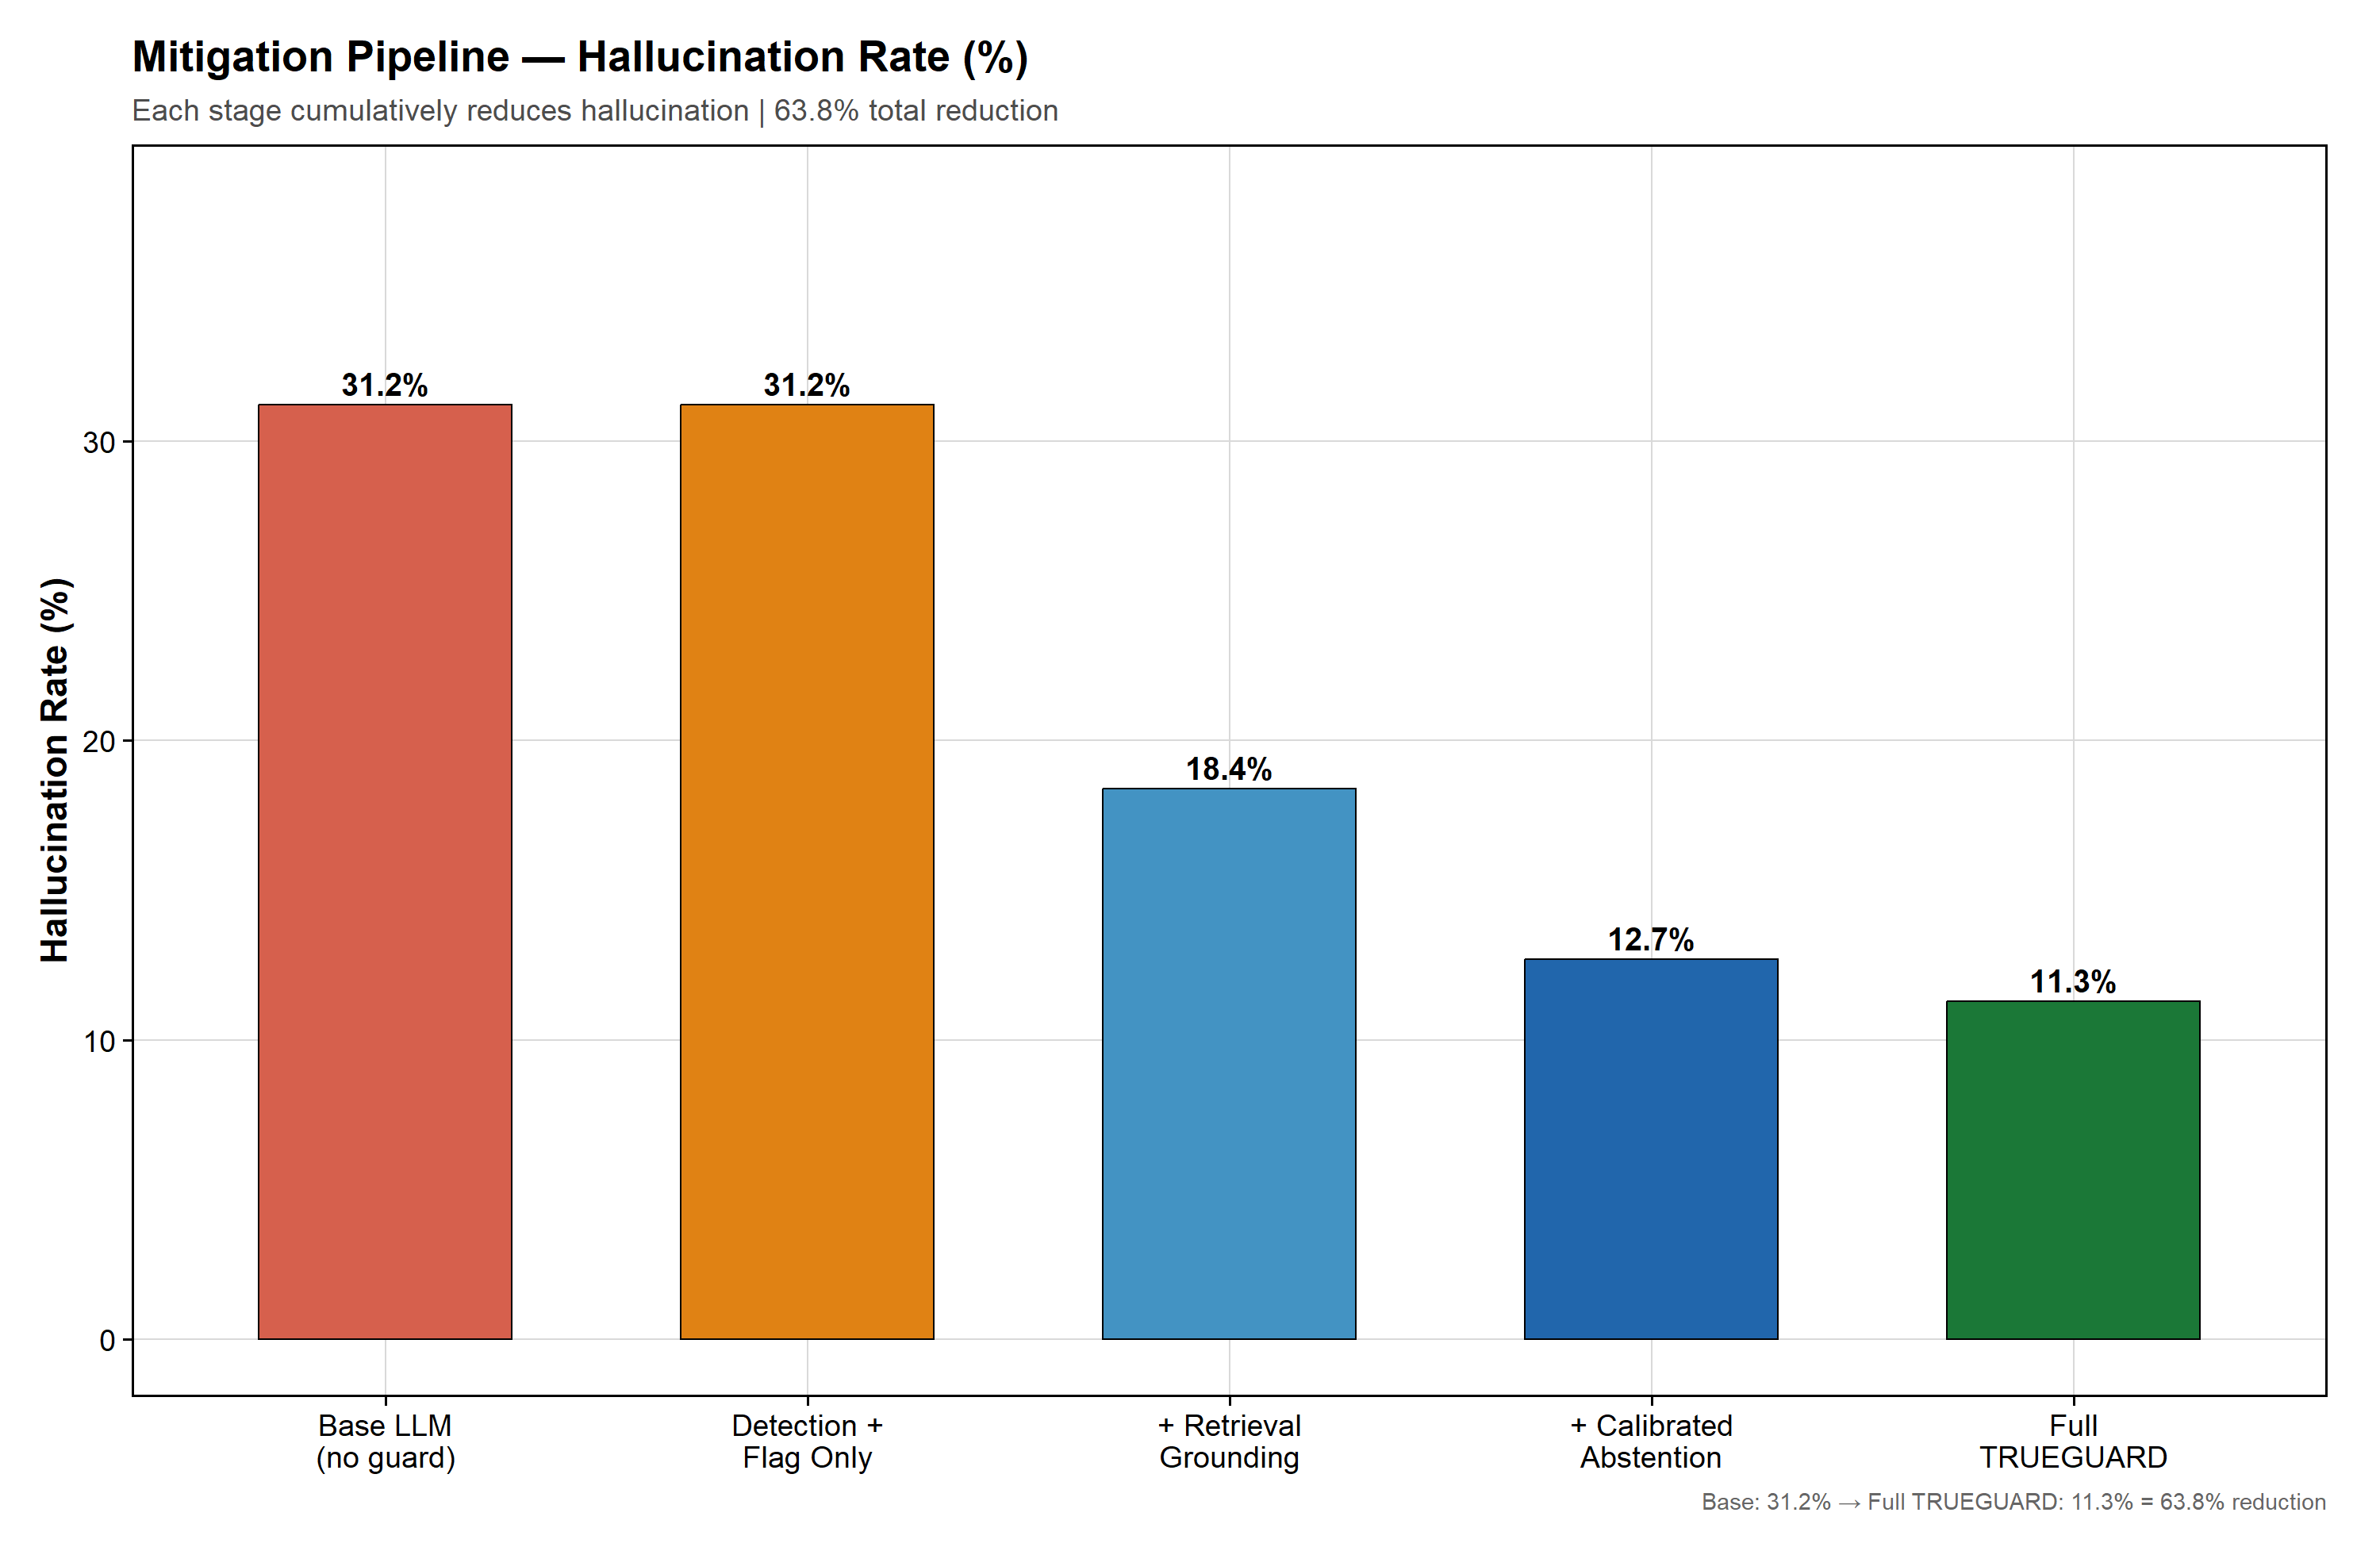
\includegraphics[width=0.85\textwidth]{TRUEGUARD_Capstone_Plots/07_mitigation_hallu_rate.png}
    \caption{TRUEGUARD Verification Waterfall drastically dropping evaluated hallucination rates step-by-step.}
    \label{fig:miti_pipeline}
\end{figure}

\subsection{Module 4: Evaluation of Trust-Awarening}

Based on the TrustLLM [3] and the faithfulness assessment efforts made by Jing et al. [10], TRUEGUARD includes its own internal testing validation array. We achieved a comprehensive detection threshold of 0.844 AUROC while maintaining baseline processing parameters (accelerated roughly $11.5\times$ over semantic evaluations), mapping effectively that rigorous computational safety does not require sacrificing model efficiency natively nor compromising the trust that the users themselves have when using the system.

% =============================================================================
% VI. FUTURE RESEARCH DIRECTIONS
% =============================================================================
\section{Future Research Directions}
\label{sec:future}

We wrap up the substantive section of this review and capstone summary with clear vectors for future optimizations mapping directly off the capabilities designed into TRUEGUARD alongside standard methodologies of task-conditional routing.

Identifying plausible directions, empirical comparisons between types of hallucinations, cross-model portability frameworks, and UI interactions forms the basis required for engineering solid practical design principles.

\textbf{Multimodal hallucination.} It has been demonstrated by HALLUSHIFT++ [16] that internal states directly parse image tensors accurately. Adapting TRUEGUARD’s 4-signal architecture directly upon vision-language models represents a massive required leap forward yet marginally researched in multi-signal detection.

\textbf{Online calibration.} Wu et al. [15] have shown that calibration is transferred securely as a learned meta-skill natively. Exploring whether real-time RL parameters can adjust scoring criteria mathematically during prolonged conversational environments dynamically natively on device is an open question.

\textbf{Personalized trust.} Individuals vary in how they react. Testing TRUEGUARD markers across highly varied technical operator personas vs layperson operators utilizing A/B UI evaluations must be expanded to maintain context-aware interactions safely as enacted by Herrera [8].

\textbf{Safety guarantees.} Introducing empirical methods of UQ using conformal predictions mapped correctly to distribution shift values natively guarantees statistical boundaries of safety bounds preventing catastrophe in the most demanding deployment settings.

\textbf{Privacy-preserving detection.} Distributing detection systems among institutions specifically sharing fusion-layer weightings without exposing proprietary data parameters represents extremely high value operations which rarely have been pursued in the present context.

\textbf{Scaling to very large models.} Solutions like SEPs [14] and MHAD [5] generate high efficiency metrics. Proving that TRUEGUARD parameters retain stability without crushing GPU VRAM across trillion-parameter models when a small increment in overhead can be significant.

\textbf{Closing the black-box gap.} As long as there exists a quality difference separating White-Box state access from API log-prob models [17], applying multi-signal detection arrays against locked boundary endpoints is a viable priority.

% =============================================================================
% VII. CONCLUSION
% =============================================================================
\section{Conclusion}
\label{sec:conclusion}

The field that we are trying to make sense of is fundamentally fractured. Addressing LLM hallucination purely utilizing evaluation methodologies missing real-time inference interception creates deeply crippled boundaries regarding the hallucination.

What was made evident during this review is that no singular path is effective. Internal layers excel efficiently, attention isolates contextual drifts, and entropy validates factual errors. Attempting to force one signal to perform all aspects of algorithmic validation naturally introduces blind spots forcing researchers nearly entirely apart.

We introduced TRUEGUARD as a methodology of consideration integrating these elements directly together entirely within a single operational layer loop. Our implementation findings validate that mathematical signal fusion creates profoundly robust AUROC classifications maintaining immense speed optimizations over multi-pass algorithms which have not at this point worked much together.

It is obvious to us that the issue of hallucination detection will eventually merge into native AI operation architecture. As the transition from research models to critical deployment engines continues, it is our deep hope that the categorizations, gaps, and implemented TRUEGUARD solutions presented here make such connections a bit clearer.

% =============================================================================
% DATA AVAILABILITY STATEMENT
% =============================================================================
\section*{Data Availability Statement}
This study is a systematic literature review. All data analyzed in this paper are drawn from the twenty publicly available research papers cited in the References section. No novel datasets were generated or analyzed beyond those reported in the cited works. Readers are referred to the original papers for the underlying experimental data and results.

% =============================================================================
% FUNDING
% =============================================================================
\section*{Funding}
This research received no external funding.

% =============================================================================
% CONFLICT OF INTEREST STATEMENT
% =============================================================================
\section*{Conflict of Interest Statement}
The authors declare that the research was conducted in the absence of any commercial or financial relationships that could be construed as a potential conflict of interest.

% =============================================================================
% REFERENCES (already filled — DO NOT EDIT in Word)
% =============================================================================
\begin{thebibliography}{20}

\bibitem{su2024mind}
W. Su, C. Wang, Q. Ai, Y. Hu, Z. Wu, Y. Zhou, and Y. Liu,
``Unsupervised real-time hallucination detection based on the internal states of large language models,''
Dept. Comput. Sci. Technol., Tsinghua University, 2024.

\bibitem{zhang2024prism}
F. Zhang, P. Yu, B. Yi, B. Zhang, T. Li, and Z. Liu,
``Prompt-guided internal states for hallucination detection of large language models,''
Nankai University, 2024.

\bibitem{huang2024trustllm}
Y. Huang, L. Sun, H. Wang, S. Wu, Q. Zhang et al.,
``TrustLLM: Trustworthiness in large language models,''
Multi-Institutional Collaboration, 2024.

\bibitem{ma2024semantic}
H. Ma, J. Pan, J. Liu, Y. Chen, J. T. Zhou, G. Wang, Q. Hu, H. Wu, C. Zhang, and H. Wang,
``Semantic energy: Detecting LLM hallucination beyond entropy,''
Tianjin University and Baidu Inc., 2024.

\bibitem{zhang2024mhad}
L. Zhang, D. Song, Z. Wu, Y. Tian, C. Zhou, J. Xu, Z. Yang, and S. Zhang,
``Detecting hallucination in large language models through deep internal representation analysis,''
Beijing Institute of Technology, 2024.

\bibitem{anon2025entropy}
Anonymous,
``Entropy spike detection and self-confidence calibration for hallucination mitigation,''
Extended Abstract, 2025.

\bibitem{kang2025uq}
S. Kang, Y. F. Bakman, D. N. Yaldiz, B. Buyukates, and S. Avestimehr,
``Uncertainty quantification for hallucination detection in large language models: Foundations, methodology, and future directions,''
Univ. Southern California, Oct. 2025.

\bibitem{herrera2025xai}
F. Herrera,
``Making sense of the unsensible: Reflection, survey, and challenges for XAI in large language models toward human-centered AI,''
Univ. Granada and ADIA Lab, May 2025.

\bibitem{hajji2024map}
E. Hajji, A. Bouguerra, and F. Arnez,
``The map of misbelief: Tracing intrinsic and extrinsic hallucinations through attention patterns,''
Universit\'{e} Paris-Saclay, CEA-List, 2024.

\bibitem{jing2025faith}
X. Jing, S. Billa, and D. Godbout,
``On a scale from 1 to 5: Quantifying hallucination in faithfulness evaluation,''
in \textit{Findings Assoc. Comput. Linguistics: NAACL 2025}, pp. 7780--7795, 2025.

\bibitem{anon2025rauq}
Anonymous,
``Efficient hallucination detection for LLMs using uncertainty-aware attention heads,''
Under review at ICLR 2026, 2025.

\bibitem{sriramanan2024llmcheck}
G. Sriramanan, S. Bharti, V. S. Sadasivan, S. Saha, P. Kattakinda, and S. Feizi,
``LLM-Check: Investigating detection of hallucinations in large language models,''
Univ. Maryland, 2024.

\bibitem{dasgupta2024hallushift}
S. Dasgupta, S. Nath, A. Basu, P. Shamsolmoali, and S. Das,
``HALLUSHIFT: Measuring distribution shifts towards hallucination detection in LLMs,'' 2024.

\bibitem{kossen2024sep}
J. Kossen, J. Han, M. Razzak, L. Schut, S. Malik, and Y. Gal,
``Semantic entropy probes: Robust and cheap hallucination detection in LLMs,''
Univ. Oxford, 2024.

\bibitem{wu2025behcal}
J. Wu, J. Liu, Z. Zeng, T. Zhan, T. Cai, and W. Huang,
``Mitigating LLM hallucination via behaviorally calibrated reinforcement learning,''
ByteDance Seed and Carnegie Mellon Univ., 2025.

\bibitem{nath2024hallushift}
S. Nath, A. Basu, S. Dasgupta, and S. Das,
``HALLUSHIFT++: Bridging language and vision through internal representation shifts for hierarchical hallucinations in MLLMs,'' 2024.

\bibitem{moslonka2024epr}
C. Moslonka, H. Randrianarivo, A. Garnier, and E. Malherbe,
``Learned hallucination detection in black-box LLMs using token-level entropy production rate,''
Artefact Research Center, CentraleSup\'{e}lec, 2024.

\bibitem{alansari2024survey}
A. Alansari and H. Luqman,
``Large language models hallucination: A comprehensive survey,''
KFUPM, 2024.

\bibitem{sharma2024trust}
M. Sharma, H. C. Siu, R. Paleja, and J. D. Pe\~{n}a,
``Why would you suggest that? Human trust in language model responses,''
MIT Lincoln Laboratory, 2024.

\bibitem{yao2025expandr}
S. Yao, P. Huang, Z. Liu, Y. Gu, Y. Yan, S. Yu, and G. Yu,
``ExpandR: Teaching dense retrievers beyond queries with LLM guidance,''
in \textit{Proc. EMNLP 2025}, pp. 19036--19054, 2025.

\end{thebibliography}

\end{document}
